%&latex
\documentclass[a4paper]{article}

\frenchspacing

\usepackage[cp1250]{inputenc}
\usepackage[czech]{babel}

\usepackage{a4wide}
\usepackage{amsmath, amsthm, amssymb, amsfonts}
\usepackage[mathcal]{eucal}
\usepackage{graphicx}
\usepackage{url}
\usepackage{color}
\usepackage{wrapfig}
\usepackage{capt-of}
\usepackage{float}
\usepackage{ifthen}
\usepackage{subfig}
\usepackage[normalem]{ulem}


% sirka a vyska textu nastavena jako papir, vsechny okraje vynulovany a pridano 20pt na kazdou stranu
% horizontalni rozmery
\setlength{\textwidth}{\paperwidth}
\addtolength{\textwidth}{-40pt}
\addtolength{\hoffset}{-1in}
\addtolength{\hoffset}{20pt}
\setlength{\oddsidemargin}{0in}
\setlength{\marginparsep}{0in}
% vertikalni rozmery
\setlength{\textheight}{\paperheight}
\addtolength{\textheight}{-60pt}
\addtolength{\voffset}{-1in}
\addtolength{\voffset}{20pt}
\setlength{\topmargin}{0in}
\setlength{\headheight}{0in}
\setlength{\headsep}{0in}


%Obrazek na miste
%pouziti
%%\obrazeknahore{adresa}{popisek}{label}
\long\def\obrazeknahore#1#2#3 {

\begin{figure}[t]
    \centering
    \includegraphics[width=0.8\textwidth]{#1}
    
    \caption{#2}
    \label{#3}
    
\end{figure}

}


%==========================================
%PEKELNA MAKRA NA ZAROVNANI OBRAZKU DOPRAVA

\makeatletter


%tohle je makro, ktere mi dovoluje obtekani i u kratkych environmentu
%ABSOLUTNE nechapu, jak to funguje, ale funguje to
%viz http://tex.stackexchange.com/questions/26078/ 
\def\odrovnej{\@@par
\ifnum\@@parshape=\z@ \let\WF@pspars\@empty \fi % reset `parshape'
\global\advance\c@WF@wrappedlines-\prevgraf \prevgraf\z@
\ifnum\c@WF@wrappedlines<\tw@ \WF@finale \fi}

\makeatother



%---
%makro, co da obrazek doprava a ostatni text ho obteka
%(bez toho predchazejiciho makra to ale poradne nebeha)
%pouziti:
%\obrazekvpravo{adresa}{popisek}{label}{procento sirky}
\long\def\obrazekvpravo#1#2#3#4{

\setlength\intextsep{-20pt}

    \begin{wrapfigure}{r}{#4\textwidth}
      \begin{center}
          \vspace{-10pt}
          
        \includegraphics[width=#4\textwidth]{#1}
        \vspace{-10pt}
        
      \end{center}
      
      \caption{#2}
      \label{#3}
      
      
    \end{wrapfigure}

\setlength\intextsep{0pt}

    
}

\long\def\obrazekvpravonocap#1#2#3{
  \setlength\intextsep{-20pt}
  
      \begin{wrapfigure}{r}{#3\textwidth}
        \begin{center}
            \vspace{-10pt}
            
          \includegraphics[width=#3\textwidth]{#1}
          \vspace{-10pt}
          
        \end{center}
        
        \label{#2}
        
        
      \end{wrapfigure}
  
  \setlength\intextsep{0pt}
}



%---
%makro pro pripady, kdy wrapfigure neco mrsi
%je to docela pekelne
%je nutne mu dat jak text vpravo, tak text vlevo
%a nevim, jestli bude 100% fungovat, ale doufam, ze jo

%pouziti:
%\obrazekvpravominipage{adresa}{popisek}{label}{procento sirky}{1 - procento sirky}{text vlevo}
\long\def\obrazekvpravominipage#1#2#3#4#5#6{

\noindent\begin{minipage}{#5\linewidth}
\vspace{0pt}
#6
\end{minipage}
\hspace{0.5cm}
\noindent\begin{minipage}{#4\linewidth}
\vspace{0pt}
\centering
\includegraphics[width=0.9\textwidth]{#1}
\captionof{figure}{#2}
\label{#3}
\end{minipage}

}

%KONEC PEKELNYCH MAKER
%=====================

\def\lebka{
\includegraphics[width=3mm]{../common/lebka}}

% makra pro poznamku u vyrokove a predikatove logiky
\def\vl{ -- ve v�rokov� logice}
\def\pl{ -- v predik�tov� logice}


%Vacsina prostredi je dvojjazicne. V pripade, ze znenie napr pozorovania je pisane po slovensky, malo by byt po slovensky aj oznacenie.

\def\ifis#1#2{\ifthenelse{\equal{#1}{0}}{}{#2}}

%\newenvironment{e}[3]{\pagebreak[2]\noindent\textbf{\ifis{#2}{$\bigstar$}#1}\ifis{#3}{\emph{~(#3)}}\par\noindent\leftskip 10pt }{\odrovnej\par\bigskip}
\newenvironment{e}[3]{\pagebreak[2]\noindent\textbf{\ifis{#2}{\lebka~}#1}\ifis{#3}{\emph{~(#3)}}\ifis{#2}{~\lebka}\par\noindent\leftskip 10pt }{\odrovnej\par\bigskip}


%obecne prostredie, ktore ma vyuzitie pri specialnych odstavcoch ako (uloha, algoritmus...) aby nevzniklo dalsich x prostredi
\newenvironment{obecne}[1]{\pagebreak[2]\noindent\textbf{#1}\par\noindent\leftskip 10pt}{\odrovnej\par\bigskip}

\newenvironment{report}{\pagebreak[2]\noindent\textbf{Report}\em\par\noindent\leftskip 10pt}{\par\bigskip}

%\newenvironment{reportN}[1]{\pagebreak[2]\noindent\textbf{Report~}\emph{(#1)}\emph\par\noindent\leftskip 10pt}{\odrovnej\par\bigskip}
\newenvironment{reportN}[1]{\pagebreak[2]\noindent\textbf{Report~}\emph{(#1)}\em\par\noindent\leftskip 10pt}{\odrovnej\par\bigskip}

\newenvironment{penumerate}{
\begin{enumerate}
  \setlength{\itemsep}{1pt}
  \setlength{\parskip}{0pt}
  \setlength{\parsep}{0pt}
  %\setlength{\topsep}{200pt}
  \setlength{\partopsep}{200pt}
}{\end{enumerate}}

\def\pismenka{\numberedlistdepth=2} %pouzit, ked clovek chce opismenkovany zoznam...

\newenvironment{pitemize}{
\begin{itemize}
  \setlength{\itemsep}{1pt}
  \setlength{\parskip}{0pt}
  \setlength{\parsep}{0pt}
}{\end{itemize}}

\definecolor{gris}{gray}{0.95}
\newcommand{\ramcek}[2]{\begin{center}\fcolorbox{white}{gris}{\parbox{#1}{#2}}\end{center}\par}


\begin{document}

\setcounter{section}{8}
\section{Vektorové priestory}

\begin{poziadavky}
\begin{pitemize}
\item Základné vlastnosti vektorových priestorov, podpriestorov generovania, lineárna závislost a nezávislosť.
\item Veta o výmene
\item Konečne generované vektorové priestory, báza.
\item Lineárne zobrazenie.
\end{pitemize}
\end{poziadavky}

\noindent Ako zdroj pre vypracovanie otázky boli použité vlastné poznámky z prednášok Lineárna algebra Jiřího Fialu a suborkové texty.

\subsection{Definície}
\begin{definicia}
Nech $(T,+,\cdot)$ je teleso a $V$ je množina (jej prvky nazývame \emph{vektory}) s binárnou operáciou $+$ a $\cdot :T \times V\to V$ je zobrazenie, potom $(V,+,\cdot)$ sa nazýva \textbf{vektorový prostor} nad telesom $T$ ak je splnených nasledujúcich 8 axiomov.
\begin{penumerate}
\item[(SA)] $\forall u,v,w \in V: \quad (u+v)+w = u+(v+w)$ \hfill\textit{(asociativita súčtu)}
\item[(SK)] $\forall u,v \in V: \quad u+v = v+u$ \hfill\textit{(komutativita súčtu)}
\item[(S0)] $\exists {\bf 0}\in V: \quad u + {\bf 0} = {\bf 0} + u = u$ \hfill\textit{(neutrálný prvok súčtu)}
\item[(SI)] $\forall u \in V \, \exists -u \in V: \quad u + (-u) = {\bf 0}$ \hfill\textit{(inverzný prvok súčtu)}
\item[(NA)] $\forall a,b \in T \, \forall u \in V: \quad (a\cdot b) \cdot u = a \cdot (b \cdot u)$ \hfill\textit{(asociativita súčinu)}
\item[(N1)] $\forall u \in V: \quad 1 \cdot u = u$ \hspace{0.5cm} kde $1 \in T$ je jednotkový prvok telesa T
\item[(D1)] $\forall a,b \in T \, \forall u \in V: \quad (a+b) \cdot u = a \cdot u + b \cdot u$ \hfill\textit{(distributivita)}
\item[(D2)] $\forall a \in T \, \forall u,v \in V: \quad a \cdot (u+v) = a \cdot u + a \cdot v$ \hfill\textit{(distributivita)}
\end{penumerate}
\end{definicia}

\pagebreak[2]
\begin{prikladySK}
\begin{pitemize}
\item $\{{\bf 0}\}$ \dots  triviálny vektorový priestor
\item $T^{n}$ aritmetický vektorový priestor dimenzie $n$ nad telesom $T$. Ide o usporiadané $n$-tice, kde + je definované predpisom
$$(x_{1}, \dots, x_{n}) + (y_{1}, \dots, y_{n}) = (x_{1} + y_{1}, \dots ,x_{n} + y_{n})$$
a násobenie predpisom
$$\alpha(x_1, \dots, x_n)=(\alpha x_1, \dots, \alpha x_n)$$
\item Z každého telesa $T$ je možné vybudovať vektorový priestor rovnakej veľkosti $V=T^{1}$
\item $\mathbb{R}$, $\mathbb{Q}$, $\mathbb{C}$, $\mathbb{Z}_{p}$, \dots, $\mathbb{R}^{2}$, $\mathbb{Q}^{2}$, \dots 
\item Matice typu $m \times n$ nad $T$ (pre konkrétne $m$, $n$)
\item Polynomy nad $T$ (napríklad obmedzeného stupňa)
\end{pitemize}
\end{prikladySK}

\subsection{Vlastnosti vektorových priestorov}

\begin{pozorovanie}
\begin{penumerate}
\item ${\bf 0}$, $-u$ sú určené jednoznačne.
\item $\forall a \in T \ \forall u \in V: \quad a \cdot {\bf 0} = 0 \cdot u = {\bf 0}$
\item $\forall a \in T \ \forall u \in V: \quad a \cdot u = {\bf 0} \ \Rightarrow\ a = 0 \ \lor\ u = {\bf 0}$.
\end{penumerate}
\end{pozorovanie}

\begin{definicia}
Nech $(V,+, \cdot )$ je vektorový priestor nad telesom T a $U \subseteq V, U \not= \emptyset$ taká, že
\begin{pitemize}
\item $\forall u,v \in U: \quad u+v \in U$ \hfill\textit{(uzavretosť na súčet)}
\item $\forall u \in U \, \forall a \in T: \quad a \cdot u \in U$ \hfill\textit{(uzavretosť na súčin)}
\end{pitemize}
potom $(U,+, \cdot )$ nazývame \textbf{podpriestorom} $V$.
\end{definicia}

\begin{pozorovanie}
Podpriestor je tiež vektorový priestor.
\end{pozorovanie}

\begin{vetaSK}
Prienik ľubovolného systému podpriestorov je podpriestor.
\end{vetaSK}

\begin{definiciaN}{Lineárny obal, množina generátorov}
Nech $V$ je vektorový priestor nad telesom T a $X$ je podmnožina $V$, potom 
$$\mathcal{L}(X) = \bigcap\{U|X \subseteq U, U \,\mathrm{je\ podpriestor}\, V\}$$
je podpriestor $V$ generovaný $X$ nazývaný \textbf{lineárny obal $X$}. Množina $X$ sa potom nazýva \emph{systém generátorov} podpriestoru $\mathcal{L}(X)$. 

Keď $\mathcal{L}(X)=V$, potom $X$ je systém generátorov vektorového priestoru $V$.
\end{definiciaN}

\begin{definice}
\textbf{Spojení dvou podprostorů} je podprostor
$$W_1 \oplus W_2 = \mathcal{L}(W_1 \cup W_2)$$
\end{definice}

\begin{vetaSK}
Lineárny obal $\mathcal{L}(X)$ obsahuje všetky lineárne kombinácie vektorov z~X.
$$\mathcal{L}(X) = \{w\big|w = \sum_{i=1}^{n}{a_{i}u_{i}}, n \geq 0, n \,\mathrm{\textit{konečné}}, \forall i: \, a_{i} \in T, u_{i} \in X\}$$
Špeciálne v prípade, že $X=\emptyset$ a teda $n=0$, platí $\mathcal{L}(X)=\{0\}$.
\end{vetaSK}

\begin{definicia}
Nech $V$ je vektorový priestor nad telesom T, potom $n$-tica vektorov $v_{1}, \dots ,v_{n} \in V$ je \textbf{lineárne nezávislá}, ak rovnica
$$a_{1}v_{1} + a_{2}v_{2} + \dots + a_{n}v_{n} = {\bf 0}$$
má iba triviálne riešenie $a_{i} = 0$ pre všetky $i \in \{1, 2, \dots, n\}$

Nekonečná množina vektorov je lineárne nezávislá, ak každá jej konečná podmnožina je lineárne nezávislá.
\end{definicia}

\begin{pozorovanie}
$X$ je lineárne nezávislá práve keď $\forall u \in X: \, u \not\in \mathcal{L}(X \setminus \{u\})$
\end{pozorovanie}

\pagebreak[3]
\begin{veta}
\begin{penumerate}
\item Obsahuje-li systém $x_1, \dots, x_n$ nulový vektor, je závislý.
\item Obsahuje-li systém $x_1, \dots, x_n$ dva stejné vektory, je závislý.
\item Pro libovolná reálná čísla $\beta_2, \dots, \beta_n$ je systém $x_1, \dots, x_n$ lineárně závislý, právě když je systém $x_1+\sum_{i=2}^n \beta_i x_i, x_2, \dots, x_n$ lineárně závislý. \textit{(Inak povedané, ak pričítame k jednému vektoru ľubovolnú lineárnu kombináciu ostatných vektorov, nezmeníme tým ich lineárnu závislosť.)}
\end{penumerate}
\end{veta}

\begin{veta}
\begin{penumerate}
	\item Podsystém lineárně nezávislého systému je lineárně nezávislý.
	\item Nadsystém systému generátorů je systém generátorů.
\end{penumerate}
\end{veta}

\begin{definicia}
Nech $V$ je vektorový priestor. Množina $X \subseteq V$ sa nazýva \textbf{báza} vektorového priestoru $V$ ak
\begin{pitemize}
	\item je lineárne nezávislá
	\item $\mathcal{L}(X) = V$
\end{pitemize}
\textit{(Inak povedané, báza je lineárne nezávislý systém generátorov.)}
\end{definicia}

\begin{vetaSK}
Každý prvok vektorového priestoru možem vyjadriť ako lineárnu kombináciu prvkov jeho báze a toto vyjadrenie je jednoznačné.
\end{vetaSK}

\begin{definicia}
Vyjadrenie vektoru $u \in V$ vzhladom k báze $X$ sa nazýva \textbf{vektor súradníc}. Značí sa $[u]_{X}$.

$(x_{1}, \dots , x_{n}) = X$ je báza $V$, $u \in V: u = a_{1}x_{1} + a_{2}x_{2} + \dots +a_{n}x_{n}$

$[u]_{X} = (a_{1}, \dots , a_{n})$
\end{definicia}

\subsection{Veta o výmene}
\begin{lemmaN}{o výmene}
Nech $v_{1},v_{2}, \dots ,v_{n}$ je systém generátorov priestoru $V$ a pre $u \in V$ platí $u = a_{1}v_{1} + a_{2}v_{2} + \dots +a_{n}v_{n}$, potom platí 
$$\forall i: \, a_{i} \not= 0 \Rightarrow \mathcal{L}(v_{1},v_{2}, \dots, v_{i-1}, u, v_{i+1}, \dots, v_{n}) = V$$
\textit{(Inak povedané, vektor bázy ktorý sa ``podielal'' na vytvorení vektoru $u$, možme s $u$ zameniť.)}
\end{lemmaN}

\begin{dokaz}
Pre ľubovolné $w \in V$, môžme písať $w = b_{1}v_{1} + b_{2}v_{2} + \dots b_{n}v_{n}$.
Do tohoto vyjadrenia miesto $v_{i}$ dosadíme vyjadrenie $v_i$ z rovnice $u = a_{1}v_{1} + a_{2}v_{2} + \dots + a_{n}v_{n}$, čím dostaneme vyjadrenie ľubovolného $w$ pomocou $v_{1},v_{2}, \dots, v_{i-1}, u, v_{i+1}, \dots, v_{n}$, z čoho výplýva, že tieto vektory sú tiež systém generátorov.
\end{dokaz}

\pagebreak[3]
\begin{vetaSKN}{Steinitzova o výmene}
Nech $V$ je vektorový priestor, $X \subseteq V$ je lineárne nezávislá a $Y \subseteq V$je konečný systém generátorov. Potom existuje $Z \subseteq V$ také, že
\begin{pitemize}
	\item $|Z| = |Y|$
	\item $\mathcal{L}(Z) = V$
	\item $Z \setminus X \subseteq Y$
	\item $X \subseteq Z$
\end{pitemize}
\textit{(V krátkosti povedané - každý nezávislý systém vektorov $X$ je možné, pridaním vektorov zo systému generátorov $Y$, rozšíriť na systém generátorov $V$.)}
\end{vetaSKN}

\begin{dokaz}
Ak $X \subseteq Y$ sme hotoví a $Z=Y$.
Inak vezmeme $Y$ a postupne do neho začneme pridávať prvky z $X \setminus Y$.
Pri každom pridaní, podľa lemmy o výmene, jeden prvok z tejto množiny odstránime. Po poslednej iterácii získame hľadané $Z$.

(Pri každej iterácií vyhadzujeme jeden prvok, ktorý nepatrí do $X$, pretože $X$ je lineárne nezávislá.)
\end{dokaz}

\begin{dosledok}
Ak má $V$ konečnú bázu, majú všetky bázy rovnakú veľkosť.
\end{dosledok}

\begin{dosledok}
Ak má $V$ konečnú bázu, potom môžme každú lineárne nezávislú množinu $X$ doplniť na bázu.
\end{dosledok}

\begin{definicia}
Veľkosť bázy konečne generovaného priestoru $V$ sa nazýva \textbf{dimenzia} priestoru $V$. Značíme $\dim(V)$.
\end{definicia}

\begin{veta}
Buďte $W_1, W_2$ konečně generované podprostory vektorového
prostoru $V.$ Potom
$$\dim W_1+\dim W_2 = \dim(W_1 \cap W_2)+\dim(W_1 \oplus W_2)$$
\end{veta}

\subsection{Lineárne zobrazenie}

\begin{definiceN}{lineární zobrazení}
Mějme vektorové prostory $V,W$. Řekneme, že zobrazení $f: V \to W$ je \textbf{lineární}, jestliže pro libovolná $x,y \in V$ a $a, b \in T$ platí
$$f(a \cdot x + b \cdot y) = a \cdot f(x) + b \cdot f(y)$$
\end{definiceN}

\begin{definiceN}{lineární operátor}
Lineární zobrazení $f: V \rightarrow V$ se nazývá \emph{lineární operátor}.
\end{definiceN}

\begin{priklady}
\begin{penumerate}
    \item Identické zobrazení $V$ na $V$ (to je příklad lineárního operátoru).
    \item Buď $\alpha$ pevné reálné číslo. Zobrazení $V \to V$ dané předpisem $x \to \alpha x.$
    \item Derivace je lineární zobrazení z množiny reálných spojitých funkcí $C_1(J)$ do množiny reálných funkcí $F(J).$
    \item V $\mathbb{R}^2$ jsou lineární zobrazení např. zrcadlení $(x,y)\mapsto(-x,y)$ nebo zkosení $(x,y)\mapsto(x+y,y)$.
\end{penumerate}
\end{priklady}

\begin{definiceN}{Hodnost lineárního zobrazení}
Pro lineární zobrazení $f:U\to V$ mezi dvěma vekt. prostory definujeme \emph{jádro zobrazení} ($\mathrm{Ker\ }f$) jako množinu $\mathrm{Ker\ }f=f^{-1}[\{0\}]$. \emph{Obraz} zobrazení $f$ ($\mathrm{Im\ }f$) je množina $\mathrm{Im\ }f=f[U]$. Jako \emph{hodnost zobrazení} $f$ označíme číslo $\mathrm{dim}(\mathrm{Ker\ }f)$.
\end{definiceN}


\begin{vetaN}{Základní vlastnosti lineárního zobrazení}
Nechť $f: V \rightarrow W$ je lineární zobrazení. Potom platí:
\begin{penumerate}
	\item $f(\mathbf{0}_V) = \mathbf{0}_W$
	\item $\mathrm{Im\ }f$ je podprostor prostoru W
	\item $\mathrm{Ker\ }(f)$ je podprostor prostoru V
	\item $f$ je prosté, právě když $\mathrm{Ker\ }(f) = \{0\}$
	\item je-li $\dim V = \dim W$ a je-li zobrazení $f$ prosté, potom je $f$ bijekce a inversní zobrazení $f^{-1}: W \rightarrow V$ je opět lineární.
\end{penumerate}
\end{vetaN}

\begin{vetaN}{O dimenzi obrazu a jádra}
Pro $f:U\to V$ mezi dvěma vektorovými prostory konečné dimenze platí:
$$\mathrm{dim}(\mathrm{Ker\ }f)+\mathrm{dim}(\mathrm{Im\ }f)=\mathrm{dim}(U)$$
\end{vetaN}

\begin{vetaN}{Báze určuje lineární zobrazení}
Mějme dány vektorové prostory $V,W$ a bázi $B=b_1,\dots,b_n$ prostoru $V$. Potom pro každé lineární zobrazení $f:B\to W$ existuje právě jedno lineární zobrazení $g:V\to W$ takové, že $f(b_i)=g(b_i)\ \forall i\in\{1,\dots,n\}$.

\emph{Jiná formulace:} Pro libovolné vektory $y_1,\dots,y_n\in W$ existuje právě jedno lineární zobrazení $g:V\to W$ takové, že $g(b_i)=y_i\ \forall i\in\{1,\dots,n\}$.
\end{vetaN}


\begin{definiceN}{Isomorfismus}
Lineární zobrazení se nazývá \emph{isomorfismus}, existuje-li k němu inversní lineární zobrazení. Pokud existuje isomorfismus $V \to W$, říkáme, že prostory $V$ a $W$ jsou \emph{isomorfní}.
\end{definiceN}

\begin{veta}
Je-li lineární zobrazení bijektivní, je to isomorfismus.
\end{veta}

\begin{vetaN}{Isomorfismus vekt. prostorů nad $\mathbb{T}$}
Každý $n$-dimensionální vektorový prostor nad tělesem $\mathbb{T}$ je isomorfní vekt. prostoru $\mathbb{T}^n$ (tj. jehož prvky jsou uspořádané $n$-tice prvků z $\mathbb{T}$).
\end{vetaN}

\begin{vetaN}{Další vlastnosti lin. zobrazení}
\begin{penumerate}
    \item Je-li lineární zobrazení prosté, zachovává lineární nezávislost.
    \item Je-li na (surjekce), zachovává vlastnost \uv{být systémem generátorů}.
\end{penumerate}
\end{vetaN}

\begin{vetaN}{Skládání lineárních zobrazeni}
Nechť $f: U \rightarrow V$, $g: V \rightarrow W$ jsou lineární zobrazení. Potom složené zobrazení $g \circ f: U \rightarrow W$ definované předpisem
$$ (g \circ f)(x) = g(f(x)) \,\, \textit{pro } x \in U$$
je rovněž lineárním zobrazením.
\end{vetaN}


\begin{vetaN}{Sčítání a násobky lin. zobrazení}
Nechť $f, g$ jsou lineární zobrazení z vekt. prostoru $V$ do $W$, $\alpha$ skalár. Potom zobrazení $f+g: V \rightarrow W$ a $\alpha f: V \rightarrow W$ definovaná předpisem
$$(f+g)(x) = f(x) + g(x), \, x \in V$$
$$(\alpha f)(x) = \alpha f(x), \, x \in V$$
jsou lineární zobrazení $V$ do $W$.
\end{vetaN}

\begin{vetaN}{Množina lineárních zobrazení je vekt. prostor}
Množina lineárních zobrazení prostoru $V$ do prostoru $W$ s operacemi sčítání a násobení skalárem, definovanými v předchozí větě, tvoří vektorový prostor, který značíme $L(V,W)$.
\end{vetaN}

\begin{veta}
Nechť $\dim V=n$ a $\dim W=m$. Potom prostor $L(V,W)$ je isomorfní prostoru $\mathbb{R}^{m\times n}$. V důsledku toho je
$$\dim L(V,W) = mn$$
\end{veta}




\setcounter{section}{9}
\newpage\section{Skal�rn� sou�in}

\begin{e}{Po�adavky}{0}{0}
\begin{pitemize}
        \item Vlastnosti v re�ln�m i komplexn�m p��pad�
        \item Norma
        \item Cauchy-Schwarzova nerovnost
        \item Kolmost
        \item Ortogon�ln� dopln�k a jeho vlastnosti
\end{pitemize}
\end{e}

\subsection{Vlastnosti v re�ln�m i komplexn�m p��pad�}
\begin{e}{Definice}{0}{0}
Nech� $V$ je vektorov� prostor nad $\mathbb{C}$. Potom zobrazen� (funkce) z kart�zsk�ho sou�inu $V \times V \rightarrow \mathbb{C}$, kter� dvojici vektor� $x$ a $y$ p�irad� ��slo $\left<x,y\right>$ se naz�v� \emph{skal�rn� sou�in}, pokud spl�uje n�sleduj�c� axiomy (pro v�echny $x, x', y \in V$ a $\alpha, \beta \in \mathbb{C}$):
\begin{penumerate}
        \item $\left<x,x\right> \ge 0, \,\, \left<x,x\right> =0 \Leftrightarrow x = 0 \hfill \textit{(positivn� definitnost)}$
        \item $\left<\alpha x+\beta x', y\right> = \alpha \left<x,y\right> + \beta \left<x',y\right> \hfill \textit{(bilinearita)}$
                \begin{penumerate}
                        \item $\left<\alpha x,y\right> = \alpha \left<x,y\right>$
                        \item $\left<x+x',y\right> = \left<x,y\right> + \left<x',y\right>$
                \end{penumerate}
        \item $\left<x,y\right> = \overline{\left<y,x\right>} \hfill \textit{(symetrie - komplexn� sdru�en�)}$ \\
                \begin{e}{Pozn�mka}{0}{0}
                        Pro $V'$ nad $\mathbb{R}$ a vektory $\forall x,y \in V'$: $\left<x,y\right>=\left<y,x\right>$
                \end{e}
\end{penumerate}

Skal�rn� sou�in zna��me: $\left<x,y\right>$, $\left<x|y\right>$, $x.y$ \dots
\end{e}

\begin{e}{Pozorov�n�}{0}{0}
\begin{pitemize}
        \item $\left<x,x\right>=\overline{\left<x,x\right>}$, tedy je nutn� re�ln� ($\in\mathbb{R}$) i pro skal�rn� sou�iny nad $\mathbb{C}$
        \item $\left<x,\alpha y\right> = \overline{\left<\alpha y,x\right>} = \overline{\alpha}.\overline{\left<y,x\right>} = \overline{\alpha}.\left<x,y\right>$
        \item Skal�rn� sou�in m��e nab�vat z�porn�ch hodnot
\end{pitemize}
\end{e}

\begin{e}{Definice}{0}{0}
Ekvivalentn� definice: \emph{Skal�rn� sou�in} je pozitivn� definitn� (1) biline�rn� forma (2). V $\mathbb{R}$ nav�c symetrick� (3). V $\mathbb{C}$ nav�c forma, jej� matice je hermitovsk� (3).
\end{e}

\begin{e}{P��klady}{0}{0}
\begin{pitemize}
        \item \uv{Standardn�} skal�rn� sou�in pro $\mathbb{C}^n, \mathbb{R}^n$: $$\left<x,y\right> = \sum_{i=1}^{n} x_i \overline{y_i}$$
        \item Jin� sou�in v $\mathbb{R}^n$ definovan� pomoc� regul�rn� matice $A$ ��du $n$
                $$\left<x,y\right>=x^T A^T A y \;\;\;\;\;\; (\textit{pozorov�n�: } \left<x,x\right> = x^T A^T A x = \sum_{i=1}^n (Ax)_i^2)$$
        \item Skal�rn� sou�in ve vektorov�m prostoru $C[a,b]$ (integrovateln�ch funkc� na intervalu $[a,b]$):
                $$\left<f,g\right> = \int_a^b f(x) g(x) dx$$
\end{pitemize}
\end{e}

\subsection{Norma}

\begin{e}{Definice}{0}{Norma}
\emph{Norma} na vektorov�m prostoru V (nad $\mathbb{R}$ nebo nad $\mathbb{C}$) je zobrazen� $V \rightarrow \mathbb{R}$, kter� p�irad� vektoru $x \in V$ ��slo $\|x\|$ a spl�uje axiomy:
\begin{penumerate}
        \item $\forall x \in V: \|x\| \ge 0, \|x\|=0 \Leftrightarrow x = 0$
        \item $\forall x \in V, \forall \alpha \in \mathbb{C} (\mathbb{R}): \|\alpha x\| = |\alpha|.\|x\|$
        \item $\forall x,y \in V: \|x\| \ge 0, \|x+y\| \le \|x\| + \|y\| \hfill \textit{(troj�heln�kov� nerovnost)}$
\end{penumerate}
Norma $\|x\|$ m� v�znam \uv{d�lky} vektoru $x$.
\end{e}

\begin{e}{Definice}{0}{Normovan� vekt. prostor}
Vektorov� prostor s n�jakou normou naz�v�me \emph{normovan�}.
\end{e}

\begin{e}{P��klady}{0}{0}
\begin{pitemize}
\item Norma ur�en� skal�rn�m sou�inem
        $$\|x\| = \sqrt{\left<x,x\right>}$$
        \begin{e}{D�kaz}{0}{0}
                (1), (2) plyne z axiom� skal�rn�ho sou�inu, (3):
                \begin{align*}
                        \left<x,y\right>^2 \le \left<x,x\right>\left<y,y\right> & \Rightarrow & \left<x,y\right> & \le & \sqrt{\left<x,x\right> \left<y,y\right>} \\
                        & \Leftrightarrow & \left<x,x\right>+\left<y,y\right>+2\left<x,y\right> & \le & (\sqrt{\left<x,x\right>} + \sqrt{\left<y,y\right>})^2 \\
                        & \Leftrightarrow & \left<x+y,x+y\right> & \le & (\sqrt{\left<x,x\right>} + \sqrt{\left<y,y\right>})^2 \\
                        & \Leftrightarrow & \|x+y\| & \le & \|x\| + \|y\|
                \end{align*}
                Kde prvn� nerovnost je d�sledek Cauchy-Swarzovy nerovnosti...

                Ze standardn�ho skal�rn�ho sou�inu na $\mathbb{R}^n$ dostaneme euklidovskou normu (tj. \uv{d�lku} vektoru podle Pythagorovy v�ty) a euklidovskou vzd�lenost (vzd�lenost bod� $u$ a $v$ je $\|u-v\|$). Ka�d� vektorov� prostor se skal�rn�m sou�inem $\left<.,.\right>$ je normovan�m vektorov�m prostorem ($\|x\|=\sqrt{\left<x,x\right>}$), tedy i metrick�m prostorem ($d(x,y)=\|x-y\|$) a tedy i topologick�m prostorem.
        \end{e}
\item $L_1$ norma na $\mathbb{R}^n$:
        $$\|x\| = \sum_{i=1}^{n} |x_i|$$
\item $L_2$ norma na $\mathbb{C}^n$ - Euklidovsk� norma:
        $$\|x\| = \sqrt{\sum_{i=1}^{n} x_i \overline{x_i}}$$
\item $L_p$ norma na $\mathbb{R}^n$:
        $$\|x\| = \sqrt[p]{\sum_{i=1}^{n} |x_i|^p}$$
\item $L_{\infty}$ norma (stejn� jako $L_1$ norma neodpov�d� ��dn�mu skal�rn�mu sou�inu):
        $$\|x\| = \max_{i=1,\dots,n} \left( |x_i| \right)$$
\item Norma v prostoru integrovateln�ch funkc� na intervalu $[a,b]$ - $C[a,b]$
        $$\|f(x)\| = \int_a^b f^2(x) dx$$
\end{pitemize}
\end{e}


\subsection{Cauchy-Schwarzova nerovnost}


\begin{e}{V�ta}{0}{Cauchyho-Schwarzova nerovnost}
Nech� $V$ je prostor se skal�rn�m sou�inem nad $\mathbb{C}$ a $\|x\|$ je norma odvozen� ze skal�rn�ho sou�inu. Potom plat�:
$$\left|\left<x,y\right>\right| \le \|x\|\cdot\|y\| \;\;\;\;\;\; (\forall x,y \in V)$$

\begin{e}{D�kaz}{0}{0}
Pro $x=0$ nebo $y=0$ m�me $0�\le 0$.

Pro libovoln� $\alpha \in \mathbb{C}$ plat� $\|x+\alpha y\|^2 \ge 0$ (plat� i bez $( )^2$)
\begin{align*}
\|x+\alpha y\|^2 = \left<x+\alpha y, x+\alpha y\right> = \left<x, x+\alpha y\right> + \alpha \left<y, x+\alpha y\right> = \\
= \left<x,x\right> + \overline{\alpha}\left<x,y\right> + \alpha\left<y,x\right> + \alpha \overline{\alpha}\left<y,y\right>
\end{align*}
Zvol�me $\alpha = \frac{-\left<x,y\right>}{\left<y,y\right>}$ (\emph{t�m se eliminuj� $\overline{\alpha}\left<x,y\right>$ a $\alpha \overline{\alpha}\left<y,y\right>$})

Po dosazen�:
\begin{align*}
0 &\le& \left<x,x\right> + \alpha \left<y,x\right> \\
0 &\le& \left<x,x\right> - \frac{\left<x,y\right>}{\left<y,y\right>}\left<y,x\right> \\
\left<x,y\right>.\left<y,x\right> &\le& \left<x,x\right>.\left<y,y\right> \\
|\left<x,y\right>|^2 & \le & \|x\|^2 . \|y\|^2 \\
\textit{...a po odmocn�n�} \\
|\left<x,y\right>| & \le & \|x\|.\|y\|
\end{align*}

\end{e}

\begin{obecne}{Druh� mo�n� d�kaz}
\noindent Nadefinujeme prom�nnou $t\in\mathbb{R}$ a zavedeme funkci
$$p(t):=\left<u+t\cdot v,u+t\cdot v\right>=||u+tv||^2$$

\noindent
V�me: $p(t)\geq 0\ \forall t\in\mathbb{R}$ (z axiomu 1 skal. sou�inu). Z linearity plyne, �e $\left<u+tv,u+tv\right>=\left<u,u+tv\right>+t\left<v,u+tv\right>=\left<u,u\right>+t\left<u,v\right>+t\left<v,u\right>+t^2\left<v,v\right>=||u||^2+2t\left<u,v\right>+t^2||v||^2$. Tj. dost�v�me $p(t)$ jako kvadratickou funkci prom�nn� $t$:
$$p(t)=t^2||v||^2+2t\left<u,v\right>+||u||^2$$

\noindent
Proto�e $p(t)$ m� nez�porn� hodnoty na cel�m $\mathbb{R}$, mus� m�t tato rovnice max. jedno �e�en�, tj. diskriminant p�i po��t�n� ko�en� nesm� b�t kladn�:
$$D=b^2-4ac=4\left<u,v\right>^2-4||u||^2||v||^2\leq 0$$

\noindent
Po vyd�len� �ty�mi a odmocn�n� dost�v�me:
$$|\left<u,v\right>|\leq ||u||\cdot||v||$$
\end{obecne}

\begin{e}{D�sledek}{0}{0}
Platnost troj�heln�kov� nerovnosti pro normy odvozen� od skal�rn�ho sou�inu -- tj. normy odvozen� od skal�rn�ho sou�inu spl�uj� v�echny axiomy normy.
\end{e}

\begin{e}{D�sledek}{0}{0}
Nech� $x=(x_1,x_2,\dots,x_n)^T$, $y=(1,1,\dots,1)^T$ jsou dva vektory, pak pro standardn� skal�rn� sou�in plat�
\begin{align*}
|\left<x,y\right>| &= \sum_{i=1}^n x_i\cdot 1\\
\|x\| &= \sqrt{\sum_{i=1}^n x_i^2}\\
\|y\| &= \sqrt{n}
\end{align*}
po dosazen� do Cauchy-Schwarzovy nerovnosti okam�it� dostaneme nerovnost mezi aritmetick�m a kvadratick�m pr�m�rem
$$\frac{1}{n}\sum_{i=1}^{n} x_i \le \sqrt{\frac{1}{n}\sum_{i=1}^{n} x_i^2}$$
\end{e}



\begin{e}{D�sledek}{0}{0}
Ve vektorov�ch prostorech nad $\mathbb{R}$ a $\mathbb{C}$ lze definovat \emph{�hel}, sv�ran� dv�ma vektory: 
$$\cos\varphi = \frac{\left<u,v\right>}{\|u\|\ \|v\|}$$
a Cauchyho-Schwarzova nerovnost zaru�uje, �e $|\cos\varphi|\leq 1$.
\end{e}

\begin{e}{D�sledek}{0}{0}
Z takto definovan�ho �hlu mezi dv�ma vektory plyne i \emph{kosinov� v�ta}: 
$$\|u-v\|^2=\|u\|^2+\|v\|^2-2\|u\|\ \|v\|\cos\varphi$$
\end{e}
\end{e}


\subsection{Kolmost}
\begin{e}{Definice}{0}{kolm� vektory}
Vektory $x$ a�$y$�z prostoru se skal�rn�m sou�inem jsou vz�jemn� \emph{kolm�}�(\emph{ortogon�ln�}), pokud $\left<x,y\right>=0$, zna��me $x \bot y$.
\end{e}

\begin{e}{Definice}{0}{ortogon�ln� a ortonorm�ln� syst�m}
Soustava (syst�m) vektor� $v_1, \dots, v_n$ se naz�v� \emph{ortogon�ln�}, jestli�e $\left<v_i,v_j\right> = 0$ ($v_i \bot v_j$) pro $\forall i \neq j$ (tj. v�echny jej� vektory jsou navz�jem kolm�). 

\noindent
Plat�-li je�t� nav�c $\|v_i\|=1$ pro $\forall i=1,\dots,n$, jedn� se o soustavu \emph{ortonorm�ln�} (vektory jsou kolm� a nav�c maj� jednotkovou normu).
\end{e}

\begin{e}{Pozorov�n�}{0}{0}
Ka�d� syst�m nenulov�ch vz�jemn� kolm�ch vektor� (tj. i ortonorm�ln� nebo ortogon�ln�) je line�rn� nez�visl�.
\end{e}

\begin{e}{D�sledek}{0}{0}
Jestli�e ortogon�ln� syst�m generuje cel� vektorov� prostor, je jeho b�z�.
\end{e}

\begin{e}{Algoritmus}{0}{Gram-Schmidtova ortogonalizace}
Tento algoritmus zaji��uje p�eveden� libovoln� b�ze $(v_1,\dots,v_n)$ vektorov�ho prostoru $V$ na ekvivalentn� ortogon�ln� b�zi $(w_1,\dots,w_n)$. Ortonormalizace b�ze u� po jeho prob�hnut� znamen� jen vyn�soben� ka�d�ho $w_i$ ��slem $\frac{1}{\|w_i\|}$. Jeho pr�b�h:
\begin{penumerate}
    \item Zvolme $w_1 := v_1$.
    \item Pro $i$ postupn� od $1$ do $n$ opakujme:
\par\noindent
    Najdi $w_i=v_i-a_{i,1}w_1 - a_{i,2}w_2 - \dots - a_{i,i-1}w_{i-1}$ tak, aby pro $\forall j\in\{1,\dots,i\}$ platilo:
    $$w_i\bot w_j$$
    D� se uk�zat �e koeficienty $a_{i,j}$ jsou tvaru
    $$a_{i,j}=\frac{\left<v_i,w_j\right>}{\|w_j\|^2}$$
    \item Po $n$ iterac�ch dostaneme $w_1,\dots,w_n$ jako ortogon�ln� b�zi prostoru $V$.
\end{penumerate}

\textbf{Alternativn� postup - Gram-Schmidtova normalizace}:
\begin{penumerate}
        \item D�ny: $x_1,\dots,x_m \in V$ line�rn� nez�visl�.
        \item Pro $k=1,\dots,m$ prove�:
                $$y_k := x_k - \sum_{j=1}^{k-1} \left<x_k,z_j\right>z_j$$
                $$z_k := \frac{1}{\|y_k\|}y_k$$
        \item Ukon�i: $z_1,\dots,z_m$ je ortonorm�ln� syst�m ve $V$ a\\$\mathcal{L}(z_1,\dots,z_m) = \mathcal{L}(x_1,\dots,x_m)$
\end{penumerate}
\end{e}

\begin{e}{D�sledek}{0}{0}
Bu� $(v_1,\dots,v_n)$ b�ze vekt. prostoru se skal. sou�inem. Potom existuje ortonorm�ln� b�ze $(w_1,\dots,w_n)$, kdy pro ka�d� $k\in\{1,\dots,n\}$ je $\mathcal{L}(v_1,\dots,v_k)=\mathcal{L}(w_1,\dots,w_k)$. D�ky tomu se ka�d� ortogon�ln� syst�m vektor� v kone�n�dimension�ln�m vekt. prostoru se skal�rn�m sou�inem d� roz���it na ortogon�ln� b�zi (to m��eme d�ky Gram-Schmidtov� ortogonalizaci a Steinitzov� v�t� o v�m�n�).
\end{e}

\begin{e}{V�ta}{0}{Fourierovy koeficienty}
M�me-li danou n�jakou ortonorm�ln� b�zi $B=b_1,\dots,b_n$ vektorov�ho prostoru $V$, pak pro ka�d� $x\in V$ plat�:
$$x=\sum_{i=1}^n\left<x,b_i\right>b_i$$
a sou�adnice $\left<x,b_i\right>$ nazveme \emph{Fourierovy koeficienty} vektoru $x$.
\end{e}

\begin{e}{Pozn�mka}{0}{0}
Fourierovy �ady jsou sou�adnice funkc� ve vektorov�m prostoru spojit�ch funkc� na $[-\pi,\pi]$ se skal�rn�m sou�inem $\left<f,g\right>=\int_{-\pi}^{\pi}f(x)g(x)\mathrm{d}x$
\end{e}


\subsection{Ortogon�ln� dopln�k a jeho vlastnosti}
\begin{e}{Definice}{0}{0}
Nech� $V$ je mno�ina vektor� ve vektorov�m prostoru $W$ se skal�rn�m sou�inem. \emph{Ortogon�ln�m dopl�kem} $V$ (zna��me $V^{\bot}$) rozum�me mno�inu
$$V^{\bot}=\left\{v \in W; \forall x \in V: \left<v,x\right> = 0 \right\}$$
\end{e}

\begin{e}{Lemma}{0}{Vlastnosti}

Nech� $V$ je podprostor prostoru $W$ kone�n� dimenze. Potom plat�:
\begin{penumerate}
        \item $V^{\bot}$ je podprostor $W$
        \item $\dim(V^{\bot})=\dim(W)-\dim(V)$
        \item $(V^{\bot})^{\bot} = V \hfill \textit{(z roz�i�itelnosti ortogon�ln� b�ze)}$ 
        \item $V \cap V^{\bot} = \{0\}, \;\;\; V \oplus V^{\bot} = W \\ \textit{(operace} \oplus \textit{je spojen� dvou podprostor�...} \mathcal{L}(V \cup V^{\bot})\textit{)}$
        \item $U,V$ podprostory $W$. Je-li $U \subseteq V$, pak $U^{\bot} \supseteq V^{\bot}$\\
                $(x \in V^{\bot} \Leftrightarrow x \bot y \in V \Rightarrow x \bot u \in U \Leftrightarrow x \in U^{\bot})$
        \item $(U \cap V)^{\bot} = U^{\bot} \oplus V^{\bot}$
        \item $(U \oplus V)^{\bot} = U^{\bot} \cap V^{\bot}$
\end{penumerate}
\end{e}

\begin{e}{Definice}{0}{Ortogon�ln� projekce}
\emph{Ortogon�ln� projekce} vekt. prostoru $V$ na podprostor $U\subset V$ je zobrazen�, kter� ka�d�mu vektoru $v\in V$ p�i�ad� vektor $u\in U$ tak, �e 
$$\|v-u\|=\min\{\|v-w\|, w \in U\}$$
tedy vektor $u \in U$, kter� m� ze v�ech vektor� z $U$ nejmen�� vzd�lenost od $v$. Ten se pak naz�v� \emph{ortogon�ln� projekc�} vektoru $v$.
\end{e}
\newpage

\begin{e}{Report}{0}{Fiala} skal�rn� sou�in a kolmost, co� byl k�men �razu, proto�e o tom jsem toho moc nev�d�l, nicm�n�, "na to, abych v�s poslal dom� se to dou�it to nen�", tak�e za 3
\end{e}
\begin{e}{Report}{0}{Matou�ek} Skal�rn� sou�in: vlastnosti, norma, C-S nerovnost, a spol. (zadal Ml�ek, p�edv�d�l jsem Matou�kovi): Definice, jejich z�ejm� d�sledky v R a C, k �emu co slou��. Zeptal se jen co je ta ��rka nad (komplexn�m ��slem) a n�sledn� co je komplexn� sdru�en� ��slo, a cht�l rozepsat CS-nerovnost pro eukleidovsk� prostor. Zapomn�l jsem na jeden axiom skal�rn�ho sou�inu (nez�pornost $<u|u>$), to mi vytkl, a p�imhou�il oko i nad t�m,�e jsem mu zprvu tvrdil, �e plyne z ostatn�ch (spletl jsem si to s normou). Kolmost jsem stihl u� jen definovat, d�l jsem se nedostal. Je�t� jsem Matou�kovi tak trochu vnutil n�znak d�kazu CS nerovnosti (kdy� u� jsem se to u�il ;)), nebyl ale vy�adov�n. 
\end{e}
\begin{e}{Report}{0}{?} Skal�rn� sou�in, Cauchyho-Schwarzova nerovnost, Troj�heln�kov� nerovnost - zde se po m� vy�adoval d�kaz CS nerovnosti, co� jsem dal, + pak jsem m�l je�t� dok�zat tu troj�heln�kovou nerovnost z CS nerovnosti - tak� se mi to povedlo. Samoz�ejm� jsem tak� napsal axiomy skal�rn�ho sou�inu. za 1
\end{e}
\begin{e}{Report}{0}{Klazar} skal�rn� sou�in (SS, norma, C-S nerovnost, pouziti (ortogonalita)), co� jsem celkem i zvl�dnul a tak celkove cele statnice dopadly za 2:)
\end{e}
\begin{e}{Report}{0}{?} skal�rn� sou�in, norma, kolmost jsme toho moc ne�ek a co jsem �ekl, tak je�t� z p�lky �patn�. Hodnocen� matika za 3(s velkym m�nusem)
\end{e}
\begin{e}{Report}{0}{Majerech} Skal�rn� sou�in. Sta�ili v�etky defin�cie pojmov uveden�ch v zozname + p�r �al��ch vlastnost�. U CSB-nerovnosti som za�al robi� aj d�kaz, ale nepozeral na�.
\end{e}
\begin{e}{Report}{0}{Klazar} Skal�rn� prostory, Cauchyova-Schwarzova nerovnost (cht�l i jak souvis� s troj�heln�kovou nerovnost� normy), jinak definice a zn�n� sta�ily) 
\end{e}
\begin{e}{Report}{0}{Klazar} Skalarni soucin. Pak jsem zacala psat matiku, to uz bylo horsi, bo vsichni pomalu odchazeli, ja tam byla uz pekne dlouho a zaclo mne byt spatne a uz me to nebavilo. K skalarnimu soucinu jsem napsala definici, definici normy, Cauchy-Schwartzovu nerovnost + dukaz a pak par vec k ortogona a ortonormalizaci a Gramm-Schmitovu ortonormalizaci. To si jen precet a ze ok.
\end{e}
\begin{e}{Report}{0}{Fiala} Skalarni soucin, ortogonalita. Uplne vklidku, stacilo definovat pojmy, napsat neco kolem, pak polozil par praktictejsich otazek, doptal se na Fourriera vzhledem k ON bazi a proc se dela a hotovo. 
\end{e}
\begin{e}{Report}{0}{Fiala} skalarni soucin, ortogonalita. Ve druhym chtel k definici SS, ortogonality a fourierovych koeficientu slyset jeste neco jako, ze na $Z_n$ nema smysl SS zavadet, coz jsem mu nerekl a tak matika vysledna lepsi dvojka. 
\end{e}
\begin{e}{Report}{0}{Pangrac} Skalarny sucin & kolmost. Dokazat bolo treba len Cauchy Schwarzovu nerovnost, tu kolmost chcel len tak prehladovo. U dokazu tej CS nerovnosti som si nevedel spomenut na nejake technicke detaily, ale to myslim vobec nevadi. Celkovo sa nejde prilis do hlbky. Za jedna
\end{e}
\begin{e}{Report}{0}{�emli�ka} C-S nerovnost. Za�al jsem tou nerovnost�. Definoval jsem t�leso, VP, sk. sou�in a nakonec normu. Chyb�l mi jeden axiom a jin� vztah tam byl nav�c, proch�zen� a nal�z�n� bylo docela �morn�, d�kaz C-S nerovnosti jsem m�l z poloviny, ale kdy� prohl�sili, �e alfa je jen technick� z�le�itost, bylo to lep��, ne� cel� d�kaz �patn�. Cht�li d�sledky nerovnosti, t�eba jako troj�heln�kovou nebo srovn�n� pr�m�r�. Ten druh� jsme spole�n�mi silami odvodili, u� jsem byl op�t dost nerv�zn�.
\end{e}
\begin{e}{Report}{0}{Gregor} C-S nerovnost. Napsal jsem definice skalarniho soucinu a normy. U normy chtel nekolik moznych "typu" normy, tj. maximalni, manhattonska atd. coz jsem moc nevedel, musel jsem patrat v pameti jeste z dob kdy to bylo na prednasce. Pak jsem napsal CS nerovnost a ideu dukazu, na detaily jsem si nevzpomel. Potom trojuhelnikovou nerovnost. Tu jsem mel s dukazem pro R, ale on chtel i pro C. Nakonec jsem to s jeho pomoci dal do kupy. 
\end{e}
\begin{e}{Report}{0}{?} CS-nerovnost - bolo potreba definovat skalarny sucin a normu (dodatocne sa ma spytal, ci poznam nejaku normu, kt. nie je urcena skalarnym sucinom, tak som skusil tu s maximom) a potom som uviedol vetu CS-nerovnost + dokaz (spomenul som si na ten z vypracovanych otazok).
\end{e}
\begin{e}{Report}{0}{Fiala} Kolmost - �la l�pe, napsal jsem jim definice kolmosti, ortogon�ln�ho a ortonorm�ln�ho syst�mu a v�ty, �e ortogon�ln� syst�m vektor� je line�rn� nez�visl�, a tu o fourierov�ch sou�adnic�ch. K dopl�ku jsem krom� definice napsal v�tu o tom, �e j�dro matice je ortogon�ln� dopln�k jej�ho ��dkov�ho prostoru. V�e jsem p�edem dok�zal (je to jednoduch�, co� potom Fiala taky takto komentoval, ale proto�e jsem �ekal fiasko s �adami, tak jsem se rad�ji rozepsal v�c). Je�t� se ptali na n�jak� vlastnosti toho dopl�ku, Fiala cht�l hlavn� n�co o dimenz�ch, tak jsem mu napsal takov� to $dim(W dopln�k) + dim(W) = dim(V)$, je�t� ze m� vyt�hl jak z chlupat� deky, �e by se to dokazovalo n�jak p�es ortogon�ln� b�ze.
\end{e}


\setcounter{section}{10}
\newpage\def\b#1{\mathbf{#1}}
\def\Ker{\mathrm{Ker\ }}
\def\Real{\mathbb{R}}
\def\rank{\mathrm{rank}}
\def\dim{\mathrm{dim}}
\def\Span{\mathcal{L}}


\section{�e�en� soustav line�rn�ch rovnic}

\begin{e}{Po�adavky}{0}{0}
\begin{pitemize}
    \item Line�rn� mno�iny ve vektorov�m prostoru, jejich geometrick� interpretace
    \item �e�en� soustavy rovnic je line�rn� mno�ina
    \item Frobeniova v�ta 
    \item �e�en� soustavy �pravou matice 
    \item Souvislost soustavy �e�en� s ortogon�ln�m dopl�kem
\end{pitemize}
\end{e}

Pojem \uv{line�rn� mno�ina} moc pou��van� nen�, proto se dr��m v�razu \uv{afinn� podprostor}. Vypracov�no s pou�it�m pozn�mek a syllabu z line�rn� algebry Prof. Matou�ka a textu Doc. M. �adka z MU Brno k line�rn� algeb�e \\(\texttt{ftp://ftp.math.muni.cz/pub/math/people/Cadek/lectures/linearni\_algebra/LA2.pdf})\\

\subsection{Line�rn� mno�iny ve vektorov�m prostoru}

\begin{e}{Definice}{0}{line�rn� mno�ina / afinn� podprostor}
Podmno�ina vektorov�ho prostoru $V$, kter� je bu� pr�zdn�, nebo tvaru
$$\b{x}+U=\{\b{x}+\b{u}|\b{u}\in U\}$$
kde $\b{x}\in V$ a $U\subset V$ je n�jak� podprostor $V$, se naz�v� \emph{afinn� podprostor}, \emph{line�rn� mno�ina} nebo \emph{line�l}.
\end{e}

\begin{e}{Pozn�mka}{0}{Nejednozna�nost ur�en� afinn�ho podprostoru}
Jeden afinn� podprostor je mo�n� ur�it v�ce zp�soby, nap�. pro vektorov� prostor $V$ s vektorem $\b{v}$ a jeho podprostorem $U$ d�vaj� $\b{v}+U$ a $2\b{v}+U$ stejn� afinn� podprostor.
\end{e}

\begin{e}{V�ta}{0}{Afinn� podprostor ur�uje vekt. prostor}
M�jme n�jak� afinn� podprostor $F$ ve vektorov�m prostoru $V$. Je-li d�no:
\begin{align*}
    F &= U + \b{x} \\
    F &= U' + \b{x'}
\end{align*}
pak jist� $U=U'$.

\begin{e}{D�kaz}{0}{0}
Ozna��me $\tilde{U}=\{\b{y}-\b{z}|y,z\in F\}$ a dok�eme, �e $\tilde{U}=U$ i $\tilde{U}=U'$.
\end{e} 
\end{e}

\begin{e}{V�ta}{0}{Lin. zobrazen� ur�uje afinn� podprostor}
Budi� d�no line�rn� zobrazen� $f:U\to V$ mezi n�jak�mi dv�ma vekt. prostory. Pro libovoln� $b\in f[U]$ potom plat�:
$$f^{-1}(\b{b})=\{\b{u}\in U|f(\b{u})=\b{b}\}=\{\b{x}_0 + \Ker f\}$$
kde $x_0$ je libovoln� vektor z mno�iny $f^{-1}(\b{b})$ a $\Ker f$ je j�dro zobrazen� $f$ (tj. $\Ker f=f^{-1}(\b{0})$).

\begin{e}{D�kaz}{0}{0}
Plyne z faktu, �e $\Ker f$ je vektorov� podprostor $U$ a z linearity $f$.
\end{e}
\end{e}

\subsection{Geometrick� interpretace}

\begin{e}{Definice}{0}{dimenze afinn�ho podprostoru, nadroviny}
\emph{Dimenzi} afinn�ho podprostoru $\b{x}+U$, kde $U\subseteq V$ je vektorov� podprostor n�jak�ho vekt. prostoru $V$, definujeme jako $\dim(U)$. 

Jednodimension�n� afinn� podprostor se naz�v� \emph{p��mka}, dvoudimension�ln� \emph{rovina}, $n-1$-dimension�ln� afinn� podprostor $n$-dimension�ln�ho prostoru se jmenuje \emph{nadrovina}.
\end{e}

\begin{e}{Pozn�mka}{0}{0}
Tot� plat� pro afinn� podprostory v $n-$rozm�rn�m eukleidovsk�m geometrick�m prostoru -- tak�e nap�. roviny nebo p��mky v trojrozm�rn�m eukleidovsk�m prostoru jsou afinn� podprostory.
\end{e}

\begin{e}{Definice}{0}{Afinn� kombinace bod�}
$\b{a},\b{b}$ bu�te dva body (vektory) ve vektorov�m prostoru $V$ nad t�lesem $T$. Potom pro $\alpha,\beta\in T$ line�rn� kombinace
$$\alpha\b{a}+\beta\b{b},\ \alpha+\beta=1_T$$
ur�uj�c� nadrovinu se naz�v� \emph{afinn� kombinace bod�}. Afinn� kombinace n�kolika bod� $\b{a}_1,\dots,\b{a}_k$ jsou pro $\alpha_i\in T$ body 
$$\sum_{i=1}^k\alpha_i\b{a}_i,\ \sum_{i=1}^k\alpha_i=1_T$$
\end{e}

\begin{e}{V�ta}{0}{Geometrick� vyj�d�en� afinn�ho podprostoru}
V afinn�m podprostoru $F$ n�jak�ho vekt. prostoru $V$ le�� s ka�d�mi $k$ body $\b{f}_1 \ldots \b{f}_k \in F$ i jejich afinn� kombinace. Naopak ka�d� mno�ina $F$ ve vekt. prostoru $V$, v n� pro ka�d� dva body le�� i jejich afinn� kombinace, je afinn� podprostor.

\begin{e}{D�kaz}{0}{0}
$F=\{U+\b{x}\}$ pro n�jak� podprostor $U\subset V$. Potom $$\forall i\in\{1,\dots,k\}:\b{f}_i=\b{x}+\b{u}_i$$ pro n�jak� $\b{u}_i\in U$. Plat�:
$$\sum_{i=1}^k(\b{x}+\b{u}_i)\alpha_i = \sum_{i=1}^k\alpha_i\b{x} + \sum_{i=1}^k\alpha_i\b{u}_i = 1\cdot\b{x} + \sum_{i=1}^k\alpha_i\b{u}_i\in F$$

Opa�n� zvolme $\b{u}\in F$, potom $F=\b{u}+\{\b{v}-\b{u},\b{v}\in F\}$ a sta�� dokaz�t, �e $U=\{\b{v}-\b{u},\b{v}\in F\}$ je podprostor $V$ (uzav�enost na skal�rn� n�sobky a sou�ty).
\end{e}
\end{e}


\subsection{�e�en� soustavy rovnic je line�rn� mno�ina}

\begin{e}{Definice}{0}{Maticov� z�pis soustavy rovnic}
Uva�ujme soustavu $m$ line�rn�ch rovnic o $n$ nezn�m�ch ve tvaru:
$$\begin{matrix}
a_{1,1}x_1 &+ a_{1,2}x_2 &+ \dots &+ a_{1,n}x_n &=& b_1 \\
a_{2,1}x_1 &+ a_{2,2}x_2 &+ \dots &+ a_{2,n}x_n &=& b_2 \\
    \vdots &             &        &  \vdots     & & \vdots \\
a_{m,1}x_1 &+ a_{m,2}x_2 &+ \dots &+ a_{m,n}x_n &=& b_m \\
\end{matrix}$$
Takovou soustavu lze zapsat jako 
$$A\b{x}=\b{b}$$
kde 
\begin{pitemize}
    \item $A$ je \emph{matice soustavy} typu $m\times n$ (s $m$ ��dky a $n$ sloupci), kde na sou�adnic�ch $[i,j]$ je koeficient $a_{i,j}$,
    \item $\b{b}$ je sloupcov� vektor prav�ch stran (matice typu $m\times 1$) a
    \item $\b{x}$ je sloupcov� vektor nezn�m�ch (matice typu $n\times 1$)
\end{pitemize}
Maticov� sou�in $A\b{x}=\b{b}$ z�ejm� d�v� stejn� v�sledek jako explicitn� z�pis soustavy.
\end{e}



\begin{e}{V�ta}{0}{�e�en� soustavy rovnic je afinn� podprostor}
Pro soustavu line�rn�ch rovnic $A\b{x}=\b{b}$, kde $A$ je matice typu $m\times n$, $\b{b}$ je vektor \uv{prav�ch stran} a $\b{x}$ vektor nezn�m�ch, plat�, �e mno�ina jej�ch �e�en� je
\begin{penumerate}
    \renewcommand{\labelenumi}{\alph{enumi})} 
    \item pr�zdn�
    \item tvaru $\{\b{x}_0+L\}$, kde $\b{x}_0$ je jedno z �e�en� soustavy $A\b{x}=\b{b}$ a $L$ je mno�ina v�ech �e�en� \emph{homogenn�} soustavy $A\b{x}=0$.
\end{penumerate}

\begin{e}{D�kaz}{0}{0}
Je-li $F$ mno�ina �e�en� rovnic $A\b{x}=\b{b}$ nepr�zdn�, potom plat�:
\begin{penumerate}
    \item ��dky matice $A$ generuj� n�jak� podprostor $L$, $\forall\b{u}\in L:A\b{u}=0$.
    \item jestli�e pro n�jak� $\b{l}$ plat� $A\b{l}=0$ (tedy $\b{l}\in L$) a m�m n�jak� $\b{x}_0$, pro kter� plat� $A\b{x}_0=\b{b}$, potom z distributivity n�soben� matic plyne $A(\b{x}_0+\b{l})=\b{b}$.
\end{penumerate}
\end{e}
\end{e}

\begin{e}{V�ta}{0}{Afinn� podprostor lze popsat soustavou rovnic}
Opa�n� tvrzen� plat� tak� -- ka�d� afinn� podprostor lze popsat soustavou line�rn�ch rovnic.

\begin{e}{D�kaz}{0}{0}
Ve vekt. prostoru $V$ m�jme afinn� podprostor $F=\{U+\b{v}\}$, kde $U\subseteq V$ je podprostor $V$ a $\b{x}\in V$. $\b{u}_1,\dots,\b{u}_k$ bu� b�ze $U$. Potom ka�d� $\b{x}\in F$ vyhovuje soustav� rovnic
$$\left(\begin{matrix}\b{u}_1\\\vdots\\\b{u}_k\end{matrix}\right)\b{x}=\b{v}$$
\end{e}
\end{e}

\begin{e}{D�sledek}{0}{0}
Je-li d�na soustava rovnic $A\b{x}=\b{b}$, kde matice $A$ m� $n$ ��dk�, potom j� ur�en� afinn� podprostor m� dimenzi $n - \rank(A)$.
\end{e}


\begin{e}{V�ta}{0}{(nepr�zdn�) pr�nik afinn�ch podprostor� je afinn� podprostor}
M�jme d�ny afinn� podprostory $F_1=\{U_1+\b{x}_1\}$ a $F_2=\{U_2+\b{x}_2\}$ pro n�jak� podprostory $U_1,U_2$ vektorov�ho prostoru $V$. Pokud $F_1\cap F_2\neq \emptyset$, potom $F_1\cap F_2$ je afinn� podprostor $V$.

\begin{e}{D�kaz}{0}{0}
Plyne z p�edchoz�ch v�t o vztahu afinn�ch podprostor� a soustav rovnic -- vezmeme rovnicov� popisy $F_1$ a $F_2$ a slo��me je pod sebe, t�m dostaneme rovnicov� popis dal��ho afinn�ho podprostoru (pokud dan� soustava rovnic m� �e�en�, tedy pr�nik je nepr�zdn�).
\end{e}

\begin{e}{P��klad}{0}{0}
Nap�. pr�nik p��mky a roviny v $\Real^3$ -- jeden bod -- je afinn� podprostor :-).
\end{e}
\end{e}


\subsection{Frobeniova v�ta }
 

\begin{e}{V�ta}{0}{Frobeniova}
Soustava line�rn�ch rovnic $A\b{x}=\b{b}$ (kde $A$ je matice s $n$ sloupci) m� alespo� jedno �e�en�, pr�v� kdy� plat�
$$\rank(A)=\rank((A\ \b{b}))$$
kde $(A\ \b{b})$ p�edstavuje tzv. \emph{roz���enou matici soustavy}, tj. matici $A$ s \uv{p�ilepen�m} vektorem prav�ch stran $\b{b}$ v posledn�m sloupci.
\par\medskip
\begin{e}{D�kaz}{0}{0}
$n$-tice skal�r� $\alpha_1,\dots,\alpha_n$ je �e�en�m soustavy $A\b{x}=\b{b}$, jinak zaps�no $A_1\alpha_1+\dots+A_n\alpha_n=\b{b}$, pr�v� kdy� sloupec $\b{b}$ je line�rn� kombinac� sloupc� $A_i, i\in\{1,\dots,n\}$, tedy $\b{b}\in\Span(A_1,\dots,A_n)$. To znamen�, �e $\Span(A_1,\dots,A_n,\b{b})=\Span(A_1,\dots,A_n)$ a tedy
$$\rank(A)=\dim(\Span(A_1,\dots,A_n))=\dim(\Span(A_1,\dots,A_n,\b{b}))=\rank((A\ \b{b}))$$
\end{e}
\end{e} 

\subsection{�e�en� soustavy �pravou matice }

\begin{e}{Definice}{0}{Element�rn� operace}
N�sleduj�c� t�i operace naz�v�me \emph{element�rn�mi operacemi} s matic� A (v�echny jsou ekvivalentn� vyn�soben� vhodnou regul�rn� matic� zleva):
\begin{penumerate}
    \item vyn�soben� i-t�ho ��dku ��slem $\alpha \neq 0$ \\ 
        (zaps�no formou maticov�ho n�soben� $A' = (I+(\alpha -1)e_i e_i^T)A$)
    \item vyn�soben� i-t�ho ��dku ��slem $\alpha$ a p�i�ten� k j-t�mu ��dku, $j \neq i$  \\
        (maticov� z�pis $A' = (I+\alpha e_j e_i^T)A$)
    \item v�m�na i-t�ho a j-t�ho ��dku, $i \neq j$ (je mo�n� \uv{slo�it} z p�edch�zej�c�ch dvou) \\
        (maticov� z�pis $A' = (I+(e_i - e_j)(e_j-e_i)^T) A$)
\end{penumerate}
\end{e}

\begin{e}{V�ta}{0}{O element�rn�ch operac�ch}
Element�rn� operace na roz���en� matici $(A\ \b{b})$ soustavy rovnic $A\b{x}=\b{b}$ nem�n� mno�inu �e�en� soustavy.
\par\medskip
\begin{e}{D�kaz}{0}{0}
D�kaz sta�� pro operace 1. a 2., proto�e t�et� je jejich kombinac�. Pro �pravy:
\begin{penumerate}
    \item Po �prav� jsou v�echny rovnice (��dky matice) a� na $i$-tou nezm�n�n�, tedy ka�d� $\b{x}$ �e�en� p�vodn� soustavy je spl�uje. Pro upraven� ��dek plat� $$\alpha(a_{i,1}x_1+\dots+a_{i,n}x_n)=\alpha\cdot b_i$$ co� je z�ejm� tak� spln�no. Podobn� se dok�e, �e ka�d� $\b{x}$ �e�en� upraven� matice spl�uje i v�echny rovnice p�vodn�.
    \item V�echny ��dky a� na $j$-t� jsou nezm�n�n� a pro $j$-t� ��dek plat�: 
$$\alpha(a_{i,1}x_1+\dots+a_{i,n}x_n)+(a_{j,1}x_1+\dots+a_{j,n}x_n)=\alpha b_i + b_j$$
a to je tak� spln�no. Opa�n� implikace se dok�e podobn�.
\end{penumerate}
\end{e}
\end{e}

\begin{e}{Definice}{0}{Odstup�ovan� tvar matice}
�ekneme, �e matice $A$ typu $m\times n$ je v (��dkov�) \emph{odstup�ovan�m tvaru}, jestli�e jsou spln�ny n�sleduj�c� podm�nky:
\begin{penumerate}
    \item existuje $r: 0\leq r \leq m$ takov�, �e ��dky $1,\dots,r$ jsou nenulov� a $r+1,\dots,m$ nulov�
    \item pro $j(i)=\min\{j | a_{i,j}\neq 0\}$ plat� $j(1)\leq j(2)\leq \dots\leq j(r)$
\end{penumerate}
\end{e}

\begin{e}{Algoritmus}{0}{�e�en� soustavy lin. rovnic}
Soustavu line�rn�ch rovnic $A\b{x}=\b{b}$ lze �e�it n�sledovn�
\begin{penumerate}
    \item Sestavit roz���enou matici soustavy
    \item P�ev�st pomoc� element�rn�ch �prav matici do odstup�ovan�ho tvaru
    \item Pomoc� zp�tn� substituce popsat v�echna �e�en�
\end{penumerate}
\end{e}

\begin{e}{Algoritmus}{0}{Gaussova eliminace}
\emph{Gaussova eliminace} je algoritmus pro �pravu dan� matice $A$ na odstup�ovan� tvar element�rn�mi ��dkov�mi �pravami. Postup:
\begin{penumerate}
    \item Ut��d�me ��dky podle d�lek �sek� po��te�n�ch nul vzestupn�
    \item Najdeme-li dva ��dky se stejn� dlouh�m �sekem po�. nul ($j(i)=j(i+1)$), potom k $i+1$-t�mu ��dku p�i�teme $-\frac{a_{i+1,j(i)}}{a_{i,j(i)}}$-n�sobek i-t�ho ��dku
    \item Kroky 1. -- 2. opakujeme, dokud existuj� dva ��dky se stejn� dlouh�m �sekem po�. nul.
\end{penumerate}

\noindent
Je zaru�eno, �e algoritmus skon��, proto�e s ka�d�m cyklem roste sou�et d�lek po��te�n�ch �sek� nul v�ech ��dk� minim�ln� o 1 a ten je omezen� ��slem $m\times n$. Slo�itost algoritmu je $O(m\cdot n^2)$.
\end{e}

\begin{e}{Algoritmus}{0}{Zp�tn� substituce}
Bu� $E$ roz���en� matice soustavy $A\b{x}=\b{b}$ v odstup�ovan�m tvaru (z�skan� pomoc� element�rn�ch �prav). Pokud po��te�n� �sek nul na n�jak�m ��dku m� d�lku $n$ (tedy nenulov� ��slo je jen ve sloupci prav�ch stran), soustava nem� �e�en�. Jinak nazveme \emph{b�zov� prom�nn�} ty, v jejich� sloupci je v n�jak�m ��dku prvn� nenulov� ��slo ($x_{j(1)},\dots,x_{j(m)}$), ostatn� nazveme \emph{voln�}. Existuje potom jednozna�n� p�i�azen� hodnot b�zov�m prom�nn�m tak, �e dohromady tvo�� �e�en� soustavy. Ka�d� �e�en� je nav�c mo�n� z�skat touto metodou.

\medskip \noindent \emph{Postup:}

\noindent Indukc� podle $i=r,r-1,\dots,2,1$. Nech� $x_{j(i)}$ je i-t� b�zov� prom�nn� a hodnoty prom�nn�ch $x_k$ pro $k>j(i)$ jsou dan� (bu� jsou voln�, nebo vyu��v�m ind. p�edpoklad). Potom po dosazen� do $i$-t� rovnice z�sk�m 
$$0x_1+\dots+0x_{j(i)-1}+a_{i,j(i)}x_{j(i)}+\dots+a_{i,j(n)}x_n=b_i$$
tedy jednu rovnici o 1 nezn�m�, kter� m� jednozna�n� �e�en�. Libovoln� �e�en� t�to soustavy $x_1,\dots,x_n$ lze z�skat touto metodou -- sta�� nastavit voln� prom�nn� podle n�j a b�zov� vyjdou spr�vn�, proto�e jejich hodnota je ur�ena jednozna�n�. Nav�c kter� prom�nn� jsou voln� a kter� jsou b�zov� je tak� ur�eno jednozna�n� -- jinak v�dy najdu r�zn� mno�iny �e�en� (co� je pro stejnou soustavu rovnic nesmysl).
\end{e}

\begin{e}{Algoritmus}{0}{Gauss-Jordanova eliminace}
Gauss-Jordanova eliminace je varianta Gaussovy eliminace, kter� p�ev�d� matici na tzv. \emph{redukovan� odstup�ovan� tvar}, to je takov� tvar, kde v ka�d�m sloupci, p��slu�ej�c�m n�jak� b�zov� prom�nn�, je pouze jedno nenulov� ��slo. Zp�tn� substituce je pak jednodu���, ale je t�eba v�ce aritmetick�ch operac� (asymptoticky jsou v�ak algoritmy stejn�)

TODO: zkontrolovat \& doplnit podrobn�ji
\end{e}

\begin{e}{Pozn�mka}{0}{0}
S �e�en�m soustav rovnic Gaussovou metodou nast�v� problem p�i strojov�ch v�po�tech -- i mal� zaokrouhlovac� chyba m��e zp�sobit velmi radik�ln� zm�nu mno�iny �e�en� (takov� matice soustav se naz�vaj� \emph{�patn� podm�n�n�}).
\end{e}

\subsection{Souvislost soustavy �e�en� s ortogon�ln�m dopl�kem}

\begin{e}{Definice}{0}{Ortogon�ln� dopln�k}
Ve vektorov�m prostoru $V$ se skal�n�m sou�inem definujeme \emph{ortogon�ln� dopln�k} mno�iny $M\subseteq V$ jako $$M^{\bot}=\{\b{v}\in V:\left<\b{v},\b{x}\right>=0\ \forall\b{x}\in M\}$$
\end{e}

\begin{e}{V�ta}{0}{Mno�ina �e�en� homogenn� soustavy je ortog. dopln�k ��dk� jej� matice}
M�jme d�nu homogenn� soustavu line�rn�ch rovnic $A\b{x}=\b{0}$ potom jej� mno�ina �e�en� je ortogon�ln� dopln�k mno�iny jej�ch ��dk� 
$$\{\b{x}|A\b{x}=\b{0}\}=\{A_1,A_2,\dots,A_n\}^{\bot}$$
p�i�em� uva�ujeme standardn� skal�rn� sou�in $\left<\b{x},\b{y}\right>=x_1y_1+\dots+x_ny_n$.
\end{e}

TODO: tady je toho dost m�lo (a� je to v�echno co jsme kdy prob�rali), jest� n�co sem doplnit ???

\begin{e}{Report}{0}{Ku�era} �e�en� soustavy line�rn�ch rovnic - K t�m rovnic�m jsem napsal necelou A4 a to sp� jen takovou okec�va�ku (Gaussova eliminace, p�evod soustavy na matici apod.). K tomu jsem teda dostal p�r dopl�uj�c�ch dotaz�, ale nic z�ludn�ho (co je mno�ina �e�en�, kdy m� nehomogenn� soustava �e�en�, pro� element�rn� �pravy nem�n� mno�inu �e�en�, pak je�t� myslim vzore�ek z Cramerova pravidla). V�sledek: 1 (�pln� bez d�kaz�)
\end{e}
\begin{e}{Report}{0}{Kolman} reseni soustavy linearnich rovnic - zprasil jsem Gaussovu eliminaci (s komentarem: tohle je princip a jeste se to musi trochu, teda vlastne hodne, opodminkovat...) 
{Loebl} reseni soustav linearnich rovnic - Napsal jsem na tema dve stranky, kdyz ke mne prisel, tak nechtel nic rikat, jen si to zbezne prohlednul a chtel dopsat jeden vzorecek, dukaz zadny. Za pet minut mi psal jednicku do "formulare". 
\end{e}
\begin{e}{Report}{0}{Ku�era} co sem videl vedle kde kdosi nebyl schopen dat dohromady frobeniovu vetu tak bych dokonce rekl ze je velice trpelivy
\end{e}
\begin{e}{Report}{0}{Fiala} Frobeniova veta + ako spolu suvisi mnozina rieseni homogennych a nehomogennych matic 
\end{e}
\begin{e}{Report}{0}{�emli�ka} �e�en� soustavy lin.rovnic pomoc� matic. Soustava pomoc� matic bylo v�cem�n� pov�d�n� o Gaussov� eliminaci, kdy je jak� prostor �e�en�, co s nulov�mi ��dky atd. Uvedl jsem afinn� prostor (vektor x0+ortogon�ln� dopln�k A), tak� �e �pravou Ax=b dostanu $x=A^{-1}.b$ (inv.matice kr�t vektor prav�ch stran) a dostalo se mi ot�zky, k �emu je to dobr�. O�ek�van� odpov��: pokud je v�cero prav�ch stran, tak sta�� Gaussovu eliminaci prov�st jen jednou (ale a� do diagon�ln� matice). Taky se p. �emli�ka ptal na implementaci Gaussovy eliminace - co hroz� a jak se toho vyvarovat (numericky nestabiln� algoritmus, hroz� chyby ze zaokrouhlov�n�, kter� se propaguj�). Pou��t p�esn�j�� reprezentaci R, spec. reprezentaci Q nebo �pln� jin� algoritmus...
\end{e}
\begin{e}{Report}{0}{Fiala} Souvislost reseni soustav linearnich rovnic s ortogonalnim doplnkem. Nu coz, zacal jsem z definicemi vseho co s tim souvisi:
soustava linearnich rovnic, matice, radkovy a sloupcovy prostor, skalarni soucin, ortogonalni mnozina
Moje tuseni ze ortogonalni doplnek radkoveho prostoru souvisi s mnozinou reseni bylo spravne.
\end{e}
\newpage


\setcounter{section}{11}
\newpage\def\rank{\mathrm{rank}}
\def\Ker{\mathrm{Ker\ }}
\def\dim{\mathrm{dim}}

\section{Matice}

\begin{pozadavky}
\begin{pitemize}
	\item Matice a jejich hodnost
	\item Operace s maticemi a jejich vlastnosti
	\item Inversní matice
	\item Regulární matice, různé charakteristiky
	\item Matice a lineární zobrazení, resp. změny souřadných soustav
\end{pitemize}
\end{pozadavky}

\subsection{Matice a jejich hodnost} 

\begin{definice}
Obdélníkové schéma sestavené z reálných čísel
$$A=\left( \begin{array}{cccc} a_{11} & a_{12} & \dots & a_{1n} \\ a_{21} & a_{22} & \dots & a_{2n} \\ \vdots & \vdots & \ddots & \vdots \\ a_{m1} & a_{m2} & \dots & a_{mn} \end{array} \right)$$
nazýváme (reálnou) maticí typu $m \times n$. Prvek $a_{ij}$ se nazývá $ij$-tý \emph{koeficient} matice A. Množinu všech reálných matic typu  $m \times n$ značíme $\mathbb{R}^{m \times n}$. Je-li $m=n$, říkáme, že matice je čtvercová řádu $n$.

Podobně definujeme množinu komplexních matic typu $m \times n$ a značíme ji $\mathbb{C}^{m \times n}$, lze takto definovat množinu matic nad libovolným tělesem.
\end{definice}

\begin{definiceN}{Jednotková matice}
Čtvercová matice řádu $n$ tvaru 
$$I=\left( \begin{array}{cccc} 1 & 0 & \dots & 0 \\ 0 & 1 & \dots & 0 \\ \vdots & \vdots & \ddots & \vdots \\ 0 & 0 & \dots & 1 \end{array} \right)$$
se nazývá \emph{jednotková matice}.
\end{definiceN}

\begin{definiceN}{Nulová matice}
Čtvercovou matici $A$ typu $m\times n$, pro kterou $a_{i,j}=0\ \forall i\in\{1,\dots,m\},\forall j\in\{1,\dots,n\}$ nazveme \emph{nulová matice} a označíme $\mathbf{0}$.
\end{definiceN}



\begin{definiceN}{Prostory související s maticí}
Buď $A$ matice typu $m\times n$ nad tělesem $\mathbb{K}$. Potom jsou s ní spojené tyto vektorové prostory:
\begin{pitemize}
    \item \emph{sloupcový prostor, též sloupcový modul} -- podprostor $\mathbb{K}^m$ generovaný sloupci $A$
    \item \emph{řádkový prostor, též řádkový modul} -- podprostor $\mathbb{K}^n$ generovaný řádky $A$
    \item \emph{jádro matice} ($\Ker A$) -- podprostor $\mathbb{K}^n$ generovaný všemi řešeními soustavy $Ax=0$
\end{pitemize}

\noindent Je zřejmé, že elementární maticové úpravy nemění ani řádkový prostor, ani jádro.
\end{definiceN}

\begin{definiceN}{Hodnost matice}
Hodnost matice $A$ je maximální počet lineárně nezávislých sloupců matice $A$ (jako vektorů), značíme ji $\rank(A)$. Hodnost matice je rovna dimenzi sloupcového prostoru (to je ekvivalentní definice).
\end{definiceN}

\begin{vetaN}{O hodnosti matice}
Pro libovolnou matici $A$ typu $m\times n$ je dimenze jejího sloupcového prostoru rovna dimenzi řádkového prostoru. Tedy hodnost matice je rovna i dimenzi řádkového prostoru a platí $$\rank(A)\leq\min\{m,n\}$$

\begin{dukaz}
Pro horní trojúhelníkové matice je tato skutečnost zřejmá, dokazuje se, že Gaussova eliminace (tj. elementární maticové úpravy -- násobení vhodnou regulární maticí zleva) nemění hodnost sloupcového prostoru (při operacích s řádky).
\end{dukaz}
\end{vetaN}

\begin{vetaN}{O dimenzích maticových prostorů}
Pro matici $A$ s $n$ sloupci platí:
$$\dim(\Ker A)+\rank(A)=n$$
\end{vetaN}

\begin{poznamka}
Po provedení \emph{Gaussovy eliminace} na matici A ($\Rightarrow A^R$) je hodnost matice A rovna počtu nenulových řádků matice $A^R$.
\end {poznamka}


\begin{definiceN}{Regulární matice}
Čtvercová matice $A$ se nazývá \emph{regulární}, jestliže soustava
$$Ax=0$$
má jediné řešení $x=0$ (tzv. \emph{triviální}).

\medskip\noindent
V opačném případě se nazývá \emph{singulární} (tj. platí $Ax=0$ pro nějaký vektor $x \neq 0$).
\end{definiceN}


\subsection{Operace s maticemi a jejich vlastnosti}

\subsubsection*{Součet a násobení skalárem}

\begin{definiceN}{Sčítání}
Nechť $A,B$ jsou matice typu $m \times n$. Potom jejich \emph{součtem} $A+B$ nazýváme matici typu $m \times n$ s koeficienty $$(A+B)_{ij} = A_{ij} + B_{ij}$$ pro $i=1,\dots,m; j=1,\dots,n$. Jsou-li $A,B$ různých typů, potom součet $A+B$ není definován.
\end{definiceN}

\begin{definiceN}{Násobení skalárem}
Nechť $A,B$ jsou matice typu $m \times n$ a $\alpha$ skalár. Potom $\alpha\cdot A$ je matice typu $m \times n$ s koeficienty $$(\alpha\cdot A)_{ij} = \alpha\cdot A_{ij}$$ pro $i=1,\dots,m; j=1,\dots,n$. Nikdy nepíšeme $A\cdot\alpha$.
\end{definiceN}

\begin{lemmaN}{Vlastnosti součtu matic a násobení matic skalárem}
Nechť $A,B,C$ jsou matice typu $m \times n$ a $\alpha, \beta$ skaláry. Potom platí:
\begin{penumerate}
	\item $A+B=B+A \hfill \textit{(komutativita)}$
	\item $(A+B)+C=A+(B+C) \hfill \textit{(asociativita)}$
	\item $A+\mathbf{0}=A \hfill \textit{(existence nulového prvku)}$
	\item $A+(-1)A=\mathbf{0} \hfill \textit{(existence opačného prvku)}$
	\item $\alpha(\beta A)=(\alpha \beta)A$
	\item $1\cdot A=A$
	\item $\alpha(A+B)=\alpha A + \alpha B \hfill \textit{(distributivita)}$
	\item $(\alpha+\beta)A=\alpha A + \beta A \hfill \textit{(distributivita)}$
\end{penumerate}
Tedy prostor matic typu $m\times n$ odpovídá vektorovému prostoru.
\end{lemmaN}

\subsubsection*{Násobení}

\begin{definiceN}{Maticové násobení}
Je-li A matice typu $m \times p$ a B matice typu $p \times n$, potom $A\cdot B$ je matice typu $m \times n$ definaná předpisem $$(A\cdot B)_{ij} = \sum_{k=1}^p A_{ik} B_{kj}$$ pro $i=1,\dots,m; j=1,\dots,n$.
\end{definiceN}


\begin{lemmaN}{Vlastnosti součinu matic}
Nechť $A,B,C$ jsou matice, $\alpha$ skalár. Potom
\begin{penumerate}
	\item Jestliže součin $(AB)C$ je definován, potom i součin $A(BC)$ je definován a platí $(AB)C=A(BC)$.
	\item Jestliže $A(B+C)$ je definován, potom i $AB+AC$ je definován a platí $A(B+C)=AB+AC$.
	\item Jestliže $(A+B)C$ je definován, potom i $AC+BC$ je definován a platí $(A+B)C=AC+BC$.
	\item Je-li $AB$ definován, je $\alpha (AB)=(\alpha A)B=A(\alpha B)$
	\item Je-li $A$ typu $m \times n$, potom $I_m A=A I_n =A$.
\end{penumerate}

\noindent Násobení matic není komutativní - tj. obecně neplatí $AB=BA$.
\end{lemmaN}

\begin{vetaN}{O hodnosti součinu matic}
Pro matici $A$ typu $m\times p$ a matici $B$ typu $p\times n$ platí:
$$\rank(AB)\leq \min\{\rank(A),\rank(B)\}$$

\begin{dukaz}
Řádkový prostor $AB$ je určitě podprostorem řádkového prostoru matice $B$ a sloupcový prostor $AB$ podprostorem sloupcového prostoru matice $A$.
\end{dukaz}
\end{vetaN}


\subsubsection*{Transpozice}


\begin{definice}
Pro matici $A \in \mathbb{R}^{m \times n}$ definujeme \emph{transponovanou matici} $A^T \in \mathbb{R}^{n \times m}$ předpisem $$(A^T)_{ji} = A_{ij} \, (i=1, \dots, m; j=1, \dots, n)$$
\end{definice}

\begin{lemmaN}{Vlastnosti transpozice}

\begin{penumerate}
	\item $(A^T)^T = A$
	\item jsou-li $A,B$ stejného typu, je $(A+B)^T = A^T + B^T$
	\item $(\alpha A)^T=\alpha A^T$, pro každé $\alpha \in \mathbb{R}$
	\item je-li $AB$ definován, je i $B^T A^T$ definován a platí $(AB)^T = B^T A^T$.
\end{penumerate}
\end{lemmaN}

\begin{definiceN}{Symetrická matice}
Matice A se nazývá \emph{symetrická} jestliže $A^T=A$.
\end{definiceN}

\begin{veta}
Pro každou matici $A \in \mathbb{R}^{m \times n}$ je $A^T A$ symetrická.
\end{veta}
\begin{veta}
Pro každou matici $A \in \mathbb{R}^{m \times n}$ platí $\rank(A^T)=\rank(A)$.
\end{veta}


\subsection{Inversní matice}

\begin{veta}
Ke každé regulární matici $A \in \mathbb{R}^{n \times n}$ existuje právě jedna matice $A^{-1} \in \mathbb{R}^{n \times n}$ s vlastností
$$A A^{-1} = A^{-1}A=I$$
Naopak, existuje-li k $A \in \mathbb{R}^{n \times n}$ matice $A^{-1}$ s touto vlastností, potom je A regulární.
\end{veta}

\begin{definice}
Matici $A^{-1}$ s touto vlastností nazýváme \emph{inversní maticí} k matici A.
\end{definice}

\begin{poznamka}
Inverzní matici mají tedy právě regulární matice.
\end{poznamka}
\begin{dusledek}
Je-li A regulární, je i $A^{-1}$ regulární.
\end{dusledek}

\begin{vetaN}{Inversní matice je oboustranně inversní}
Jestliže pro $A,X \in \mathbb{R}^{n \times n}$ platí $XA=I$, potom A je regulární a $X=A^{-1}$. Analogicky, jestliže $AX=I$, potom A je regulární a $X=A^{-1}$.
\end{vetaN}

\begin{veta}
Je-li $A \in \mathbb{R}^{n \times n}$ regulární, potom pro každé $b \in \mathbb{R}^n$ je jediné řešení soustavy $Ax=b$ dáno vzorcem $x = A^{-1}b$.
\end{veta}

\begin{vetaN}{Výpočet inversní matice}
Pro čtvercovou matici $A$ řádu $n$ nechť je matice $(A\ I)$ (tj. zřetězení sloupců matice $A$ a jednotkové matice $I$ řádu $n$) převedena  Gauss-Jordanovou eliminací na tvar $(I\ X)$. Potom platí: 
$$X=A^{-1}$$ 
Jestliže Gauss-Jordanova eliminace není proveditelná až do konce, potom $A$ je singulární a nemá inversní matici.

\medskip
\begin{dukaz}
Víme, že Gauss-Jordanova eliminace je vlastně opakované násobení regulárními maticemi zleva. Součin všech těchto matic označme $Q$. Označme $H_{*,j}$ $j$-tý sloupec nějaké (obecné) matice. Potom pro $j\in\{1,\dots,n\}$ platí: $(I\ X)_{*,j}=I_{*,j}=Q(A\ I)_{*,j}=(QA)_{*,j}$, tedy $QA=I$, dále platí $(I\ X)_{*,n+j}=X_{*,j}=(QI)_{*,n+j}=Q_{*,j}$, takže $Q=X$ a tedy $AX=I$.
\end{dukaz}
\end{vetaN}

\begin{vetaN}{Vlastnosti inversní matice}
Nechť $A,B \in \mathbb{R}^{n \times n}$ jsou regulární matice. Potom platí:
\begin{penumerate}
	\item $(A^{-1})^{-1} = A$
	\item $(A^{T})^{-1} = (A^{-1})^{T}$
	\item $(\alpha A)^{-1} = \frac{1}{\alpha} A^{-1} \textit{ pro }\alpha \neq 0$
	\item $(AB)^{-1} = B^{-1} A^{-1}$
\end{penumerate}
\end{vetaN}


\subsection{Regulární matice, různé charakteristiky}

\begin{vetaN}{Násobení regulární maticí a hodnost}
Pro čtvercovou regulární matici $R$ řádu $m$ a matici $A$ typu $m\times n$ platí:
$$\rank(RA)=\rank(A)$$

\medskip
\begin{dukaz}
Nerovnost \uv{$\leq$} plyne přímo z věty o hodnosti součinu matic použité pro $RA$, opačná nerovnost z téže věty, použité na matici $R^{-1}\cdot(RA)=A$.
\end{dukaz}
\end{vetaN}

\begin{vetaN}{Násobení regulárních matic}
Jsou-li $A_1,A_2,\dots,A_q \in \mathbb{R}^{n \times n}$ regulární, $q \ge 1$, potom $A_1 A_2 \dots A_q$ je regulární.

\medskip
\begin{dukaz}
Plyne přímo z předchozí věty.
\end{dukaz}
\end{vetaN}


\begin{poznamkaN}{Podmínky regularity}
Čtvercová $A \in \mathbb{R}^{n \times n}$ je regulární matice, právě když:
\begin{pitemize}
 %	\item $\det A \neq 0$ -- determinanty v sekci 12 jeste neumime
	\item Její řádky jsou lineárně nezávislé
	\item Její sloupce jsou lineárně nezávislé
	\item Její hodnost je právě $n$
	\item $A^{T}$ je regulární
	\item $A^{-1}$ je regulární
\end{pitemize}
\end{poznamkaN}

Další charakteristiky regulárních matic:
\begin{pitemize}
	\item Matice A je regulární právě když je determinant nenulový.
	\item Právě když po provedení Gaussovy-Jordanovy eliminace dostaneme jednotkovou matici.
	\item Právě když lze napsat jako součin matic $E_k \times \dots \times E_2 \times E_1 \times I_n$, kde $I_n$ je jednotková matice a $E_1 \times E_k$ jsou elementární matice (odpovídají elementárním řádkovým úpravám, které matici A převádí na redukovaný, řádkově odstupňovaný tvar).
\end{pitemize}

\subsection{Matice a lineární zobrazení, resp. změny souřadných soustav}

\begin{definice}
Nechť V, W jsou vektorové prostory nad stejným tělesem (R nebo C). Zobrazení $f: V \rightarrow W$ nazýváme \emph{lineárním zobrazením} jestliže
\begin{penumerate}
	\item $f(x+y)=f(x)+f(y)$ pro každé $x,y \in V$
	\item $f(\alpha\cdot x)=\alpha\cdot f(x)$ pro každé $x \in V$ a každý skalár $\alpha$.
\end{penumerate}
\end{definice}

\begin{definiceN}{Souřadnicový vektor}
Nechť $\mathbb{B}=(x_1,\dots,x_n)$ je báze V. Každý vektor $x \in V$ lze potom vyjádřit právě jedním způsobem jako lineární kombinaci vektorů báze $\mathbb{B}$. Potom aritmetický vektor
$$[x]_{\mathbb{B}} = \left( \begin{array}{l}\alpha_1 \\ \vdots \\ \alpha_n \end{array} \right)$$
nazýváme \emph{souřadnicovým vektorem} vektoru x v bázi $\mathbb{B}$ (a $n=\dim V$ a souřadnicový vektor \emph{závisí na výběru báze}).
\end{definiceN}


\begin{definiceN}{Matice lineárního zobrazení}
Nechť $\mathbb{B}=\{x_1, \dots, x_n\}$ je báze vektorového prostoru $V$, $\mathbb{B}'=\{y_1, \dots, y_m\}$ je báze vekt. prostrou $W$ a nechť $f: V \rightarrow W$ je lineární zobrazení. Potom pro každé $j=1, \dots, n$ lze $f(x_j)$ zapsat právě jedním způsobem ve tvaru
$$f(x_j) = \sum_{i = 1}^{m} \alpha_{ij} y_j.$$

Matice $A=(\alpha_{ij}) \in \mathbb{R}^{m \times n}$ se nazývá maticí lineárního zobrazení $f$ vzhledem k bázím $\mathbb{B}, \mathbb{B}'$ a značí se
$$[f]_{\mathbb{B}\mathbb{B}'}.$$
\end{definiceN}

\begin{pozorovani}
$[f]_{\mathbb{B}\mathbb{B}'}.$ je matice sestavená ze sloupců
$$([f(x_1)]_{\mathbb{B}'}, \dots, [f(x_n)]_{\mathbb{B}'}),$$
které jsou souřadnicovými vektory vektorů $f(x_1), \dots, f(x_n)$ v bázi $\mathbb{B}'$.
\end{pozorovani}

\begin{veta}
Nechť $\mathbb{B}$ je báze V, $\mathbb{B}'$ je báze W, a nechť $f: V \rightarrow W$ je lineární zobrazení. Potom pro každé $x \in V$ platí
$$[f(x)]_{\mathbb{B}'} = [f]_{\mathbb{B} \mathbb{B}'}.[x]_{\mathbb{B}},$$
kde napravo stojí maticový součin.
\end{veta}

\begin{vetaN}{Složené zobrazení a maticový součin}
Nechť $f: U \rightarrow V$, $g: V \rightarrow W$ jsou lineární zobrazení a nechť $\mathbb{B}, \mathbb{B}', \mathbb{B}''$ jsou báze U, V, W. Potom platí
$$[g \circ f]_{\mathbb{B} \mathbb{B}''}=[g]_{\mathbb{B}'\mathbb{B}''} [f]_{\mathbb{B}\mathbb{B}'}$$
kde napravo stojí maticový součin.
\end{vetaN}

\begin{vetaN}{Matice inversního zobrazení}
Je-li $f: V \rightarrow W$ isomorfismus, potom inversní zobrazení $f^{-1}: W \rightarrow V$ je rovněž isomorfismus a vzhledem k libovolným bázím $\mathbb{B}, \mathbb{B}'$ prostorů V, W platí:
$$[f^{-1}]_{\mathbb{B}' \mathbb{B}} = [f]^{-1}_{\mathbb{B} \mathbb{B}'}$$
\end{vetaN}

\begin{vetaN}{Změna souřadnic vektoru při změně báze}
Nechť jsou dány dvě báze $\mathbb{B}, \mathbb{B}'$ vektorového prostoru $V$. Potom pro každé $x \in V$ platí:
$$[x]_{\mathbb{B}'} = [\mathrm{id}_V]_{\mathbb{B} \mathbb{B}'}.[x]_{\mathbb{B}}$$

Matice $[\mathrm{id}_V]_{\mathbb{B} \mathbb{B}'}$ se nazývá \emph{maticí přechodu} od báze $\mathbb{B}$ k bázi $\mathbb{B}'$.
\end{vetaN}

\begin{poznamka}
Předchozí vzorec vyžaduje znalost hodnot vektorů staré báze $\mathbb{B}$ v nové bází $\mathbb{B}'$. Typická situace ale je, že máme jen starou bázi $\mathbb{B}$ a pomocí ní vyjádříme novou bázi $\mathbb{B}'$. V tom případě můžeme použít vzorec
$$[x]_{\mathbb{B}'} = [\mathrm{id}_V]^{-1}_{\mathbb{B}' \mathbb{B}} [x]_{\mathbb{B}}$$
\end{poznamka}


\setcounter{section}{12}
\newpage\def\sgn{\mathrm{sgn}}
\def\adj{\mathrm{adj\ }}

\section{Determinanty}

\begin{e}{Po�adavky}{0}{0}
\begin{pitemize}
\item Definice a z�kladn� vlastnosti determinantu
\item �pravy determinant�, v�po�et
\item Geometrick� smysl determinantu
\item Minory a inversn� matice
\item Cramerovo pravidlo.
\end{pitemize}
\end{e}

\subsection{Definice a z�kladn� vlastnosti determinantu}

\begin{obecne}{Neform�ln�}
V line�rn� algeb�e je \emph{determinant} zobrazen�, kter� p�i�ad� ka�d� �tvercov� matici $A$ skal�r $\det A$.

Determinantem �tvercov� matice ��du $n$ naz�v�me sou�et v�ech sou�in� $n$ prvk� t�to matice takov�ch, �e v ��dn�m z uveden�ch sou�in� se nevyskytuj� dva prvky z t�ho� ��dku ani z t�ho� sloupce. Ka�d� sou�in p�itom n�sob�me ��sly $r$ a $s$, kde $r$ p�edstavuje znam�nko permutace p��slu�n�ho po�ad� prvn�ch index� a $s$ znam�nko permutace p��slu�n�ho po�ad� druh�ch index�.
\end{obecne}

\begin{e}{Definice}{0}{permutace, znam�nko}
\emph{Permutace} je libovoln� bijekce $\sigma:X\to X$. Mno�ina \emph{invers�} n�jak� permutace $\sigma$ je $I(\sigma)=\{(i,j):i<j \ \&\ \sigma(i)>\sigma(j)\}$. Znam�nko permutace $\sgn(\sigma)$ se pak definuje jako $\sgn(\sigma)=(-1)^{|I(\sigma)|}$. Nejjednodu��� permutace -- z�m�na dvou prvk� -- se pak naz�v� \emph{transpozice}. Ta m� v�dy znam�nko $-1$ a libovoln� permutace je slo�en�m n�jak�ch transpozic. Mno�inu v�ech permutac� na mno�in� $\{1,\dots,n\}$ zna��me $S_n$.
\end{e}

\begin{e}{Pozn�mka}{0}{0}
Pro skl�d�n� permutac� plat� $\sgn(p\circ q)=\sgn(p)\sgn(q)$. Pro inversn� permutaci (inversn� zobrazen�) plat� $\sgn(p)=\sgn(p^{-1})$.
\end{e}

\begin{e}{Definice}{0}{determinant}
Nech� $A = (a_{i,j})^{n}_{i,j=1}$ je �tvercov� matice ��du $n$.
Determinant je definovan� pomoc� \emph{Leibnizova vzorce}:

$$\det A = \sum_{\sigma \in S_n}sgn(\sigma) \prod_{i=1}^n a_{i,\sigma(i)}$$
\end{e}

\begin{e}{Pozn�mka}{0}{0}
Suma se po��t� p�es v�echny permutace $\sigma$ ��sel \{1,2,\dots,n\}, tak�e tento vzorec obsahuje $n!$ (faktori�l) s��tanc�, co� jej s r�stem \emph{n} rychle �in� prakticky nepou�iteln�m pro v�po�et. V praxi se proto pou��vaj� jin� zp�soby v�po�tu.
\end{e}

\begin{e}{Pozn�mka}{0}{0}
Konkr�tn�, pro matici ��du $n$, kde:
\begin{pitemize}
\item $n=1: \det A = a_{1,1}$
\item $n=2: \det A = a_{1,1} a_{2,2} - a_{2,1} a_{1,2}$
\item $n=3: \det A = a_{1,1} a_{2,2} a_{3,3} + a_{1,3} a_{2,1} a_{3,2} + a_{1,2} a_{2,3} a_{3,1} - a_{1,3} a_{2,2} a_{3,1} - a_{1,1} a_{2,3} a_{3,2} - a_{1,2} a_{2,1} a_{3,3}$
\end{pitemize}

Mnemotechnick� pom�cka slou��c� k zapamatov�n� postupu v�po�tu determinantu t�et�ho ��du se naz�v� \emph{Sarrusovo pravidlo}:
\begin{center} 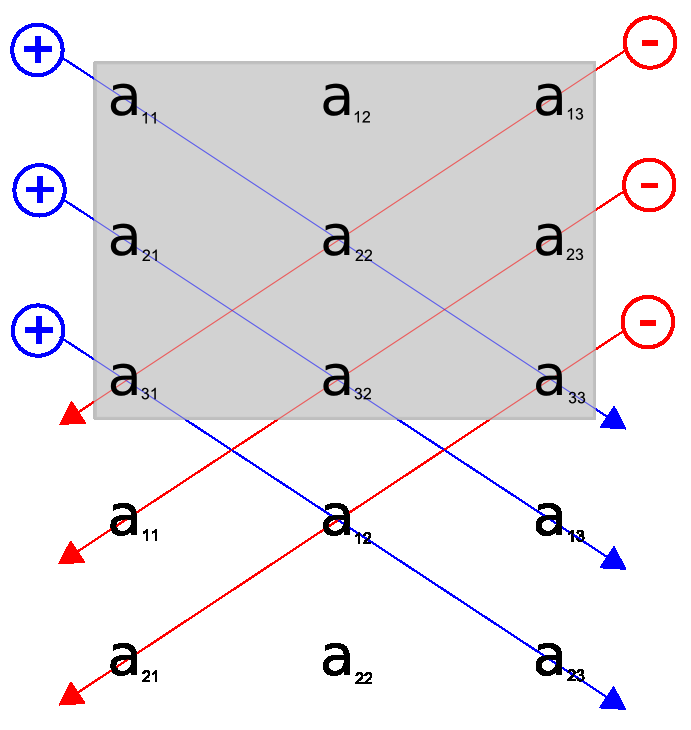
\includegraphics[width=5cm]{matematika/obrazky/sarrusovo_pravidlo.png} \end{center}
\end{e}

\begin{e}{Pozn�mka}{0}{0}
Obecn� vzorec lze tak� vyj�d�it pomoc� Levi-Civitova symbolu $\epsilon_{{j_1}{j_2}\dots{j_n}}$ jako
$$\det A = \sum_{{j_1},{j_2}, \dots ,{j_n}}\epsilon_{{j_1}{j_2} \dots {j_n}} a_{1,j_1}a_{2,j_2}  \dots  a_{n,j_n} = \sum_{{j_1},{j_2}, \dots ,{j_n}}\epsilon_{{j_1}{j_2} \dots {j_n}} a_{j_1,1}a_{j_2,2}  \dots  a_{j_n,n}$$
\end{e}

\subsubsection*{Vlastnosti determinantu}

\begin{e}{V�ta}{0}{O determinantu transponovan� matice}
Pro �tvercovou matici $A$ ��du $n$ plat�:
$$\det A=\det A^T$$

\begin{e}{D�kaz}{0}{0}
Plyne z faktu �e $\sgn(p)=\sgn(p^{-1})$:
\begin{align*}
\det(A^T) & =\sum_{p\in S_n}\sgn(p)\prod_{i=1}^n(A^T)_{i,p(i)}=\\
 & =\sum_{p\in S_n}\sgn(p)\prod_{i=1}^n a_{p(i),i}=\sum_{p^{-1}\in S_n}\sgn(p^{-1})\prod_{i=1}^n a_{i,p^{-1}(i)}=\det(A)
\end{align*}
\end{e}
\end{e}

\begin{e}{V�ta}{0}{P�erovn�n� matice}
P�erovn�n� ��dk� nebo sloupc� podle permutace $p$ nezm�n� determinant v�bec, pokud $\sgn(p)=1$ a zm�n� jen jeho znam�nko, pokud $\sgn(p)=-1$.

\begin{e}{D�kaz}{0}{0}
A bu� p�vodn� matice a B p�erovnan�:
\begin{align*}
\det(B) & =\sum_{p\in S_n}\sgn(p)\prod_{i=1}^n(B)_{i,p(i)} = \sum_{p\in S_n}\sgn(p)\prod_{i=1}^n(A)_{i,q^{-1}\left(p(i)\right)}=\\
 & =\sgn(q)\sum_{p\in S_n}\sgn(q)\sgn(p)\prod_{i=1}^n(A)_{i,q^{-1}\left(p(i)\right)}=\sgn(q)\sum_{p\in S_n}\sgn(h)\prod_{i=1}^n(A)_{i,h(i)}=\\
 & =\sgn(q)\det(A)
\end{align*}
\end{e}
\end{e}

\begin{e}{D�sledek}{0}{0}
M�-li matice dva shodn� sloupce nebo ��dky, m� automaticky nulov� determinant (p�ehozen�m pr�v� t�ch dvou ��dk� nebo sloupc� vzniknou shodn� matice se stejn�m determinantem, ale m� se zm�nit znam�nko).
\end{e}

\begin{e}{V�ta}{0}{Determinant jako line�rn� funkce}
Determinant matice $A$ je line�rn� funkc� ka�d�ho jej�ho ��dku i ka�d�ho sloupce, tj. plat�
\begin{penumerate}
    \item $$\det\left(\begin{matrix}
a_{1,1}& \dots & a_{1,n}\\
\vdots & & \vdots \\
b_{i,1}& \dots & b_{i,n}\\
\vdots & & \vdots \\
a_{n,1}& \dots & a_{n,n}\\
\end{matrix}\right)
+ \det\left(\begin{matrix}
a_{1,1}& \dots & a_{1,n}\\
\vdots & & \vdots \\
c_{i,1}& \dots & c_{i,n}\\
\vdots & & \vdots \\
a_{n,1}& \dots & a_{n,n}\\
\end{matrix}\right)
= \det\left(\begin{matrix}
a_{1,1}& \dots & a_{1,n}\\
\vdots & & \vdots \\
b_{i,1} + c_{i,1}& \dots & b_{i,n} + c_{i,n}\\
\vdots & & \vdots \\
a_{n,1}& \dots & a_{n,n}\\
\end{matrix}\right)$$
    \item $$\det\left(\begin{matrix}
a_{1,1}& \dots & a_{1,n}\\
\vdots & & \vdots \\
\kappa a_{i,n}& \dots & \kappa a_{i,n}\\
\vdots & & \vdots \\
a_{n,1}& \dots & a_{n,n}\\
\end{matrix}\right)
= \kappa \det(A)$$
\end{penumerate}

\begin{e}{D�kaz}{0}{0}
Prvn� ��st plyne z distributivity s��t�n� vzhledem k n�soben� -- ka�d� �len sumy (produkt prvk�) obsahuje jeden prvek typu $b_{i,p(i)} + c_{i,p(i)}$ pro n�jakou permutaci a ten je mo�n� rozepsat. Druh� ��st se dok�e podobn� d�ky komutativit� n�soben� -- prvek $\kappa$ je tak� obsa�en v ka�d�m �lenu sumy pr�v� jednou, tak�e je ho mo�n� \uv{vytknout}.
\end{e}
\end{e}

\begin{e}{V�ta}{0}{Determinant sou�inu matic}
Nech� $A$ a $B$ jsou �tvercov� matice stejn�ho ��du $n$ nad t�lesem $T$. Potom plat�:
$$\det(A\cdot B)=\det(A)\cdot\det(B)$$

\begin{e}{D�kaz}{0}{0}
Je-li jedna z matic singul�rn�, je jejich sou�in singul�rn� a tedy m� nulov� determinant; stejn� jako je nulov� sou�in determinant� p�vodn�ch matic. Jsou-li ob� matice regul�rn�, lze $A$ rozlo�it na n�jak� sou�in $E_1\cdot E_2\cdot\dots\cdot E_k$ element�rn�ch matic. Potom 
\begin{align*}
\det(AB) & = \det(E_1E_2\dots E_k B)=\det(E_1)\cdot\det(E_2\dots E_k B)\\
& =\det(E_1)\det(E_2)\dots\det(E_k)\det(B)=\det(A)\det(B)
\end{align*}
proto�e v�me, jak�m zp�sobem element�rn� �pravy (ekvivalent element�rn�ch matic ve vzorci) m�n� determinant.
\end{e}
\end{e}

\begin{e}{D�sledek}{0}{0}
�tvercov� matice je regul�rn�, pr�v� kdy� m� nenulov� determinant.
\end{e}

\subsection{�pravy determinant�, v�po�et}

\begin{obecne}{Gaussova eliminace}
Gaussova metoda spo��v� v proveden� takov�ch �prav matice, kter� nem�n� hodnotu determinantu, ale zjednodu�� v�po�et jeho hodnoty. C�lem prov�d�n�ch �prav je z�skat troj�heln�kovou matici \textbf{A} (kde pro $i > j$ je $a_{i,j} = 0$), nebo� pro troj�heln�kov� matice plat�

$$\det A = a_{1,1} a_{2,2}  \dots  a_{n,n}$$

\noindent
tzn. determinant je roven sou�inu prvk� hlavn� diagon�ly matice.

\noindent
P�i �prav�ch matice pro v�po�et determinantu postupujeme podle t�chto pravidel:
\begin{pitemize}
\item Pokud \textbf{B} vznikne z \textbf{A} v�m�nnou dvou ��dku nebo sloupc� potom $\det B = -\det A$
\item Pokud \textbf{B} vznikne z \textbf{A} vyn�soben�m ��dku nebo sloupce skal�rem c, potom $\det B = c.\det A$
\item Pokud \textbf{B} vznikne z \textbf{A} p�i�ten�m n�sobku jednoho ��dku k jin�mu, nebo p�id�n�m n�sobku sloupce k jin�mu sloupci potom $\det B = \det A$
\end{pitemize}

\noindent
Opakovan�m pou�it�m uveden�ch pravidel p�evedeme matici na troj�heln�kovou a pro tu pot� snadno spo�teme determinant.
\end{obecne}



\subsection{Geometrick� smysl determinantu}

\begin{obecne}{Matice ��du 2}
Absolutn� hodnotu determinantu matice ��du 2
$$\det\left(
\begin{array}{cc}
a & b\\
c & d
\end{array}
\right) = ad - bc
$$
lze interpretovat jako obsah rovnob�n�ku s vrcholy v bodech $(0,0)$, $(a,c)$, $(b, d)$ a $(a+b, c+d)$. Znam�nko determinantu ur�uje vz�jemnou orientaci vektor� $(a,c)$, $(b, d)$. $\det A$ je kladn�, pokud �hel mezi vektory $(a,c)$, $(b, d)$ m��en� v kladn�m sm�ru (tedy proti sm�ru hodinov�ch ru�i�ek) men�� ne� $\pi$, a z�porn�, pokud je tento �hel v�t�� ne� $\pi$.
\end{obecne}

\begin{obecne}{Matice ��du 3}
Podobn� geometrick� v�znam jako pro matici ��du 2 najdeme i pro matice $B = (b_{i,j})$ ��du 3. ��dkov� vektory

$$b_1 = (b_{1,1}, b_{1,2}, b_{1,3}), b_2 = (b_{2,1}, b_{2,2}, b_{2,3}), b_3 = (b_{3,1}, b_{3,2}, b_{3,3})$$

ur�uj� v t��dimenzion�ln�m prostoru rovnob�nost�n, jeho� objem je roven $\left| \det B \right|$. Pokud je $\det B$ kladn�, tak je posloupnost vektor� $b_1, b_2, b_3$ pravoto�iv�, a levoto�iv�, pokud je $\det B$ z�porn�.
\end{obecne}

\begin{obecne}{Matice vy���ch ��d�}
I v re�ln�ch prostorech vy���ch ��d� lze determinant ch�pat jako objem obecn�ho \emph{n}-rozm�rn�ho rovnob�nost�nu, p��padn� jako pravoto�ivost, respektive levoto�ivost posloupnosti $b_1, b_2,  \dots , b_n$.
\end{obecne}

\begin{e}{Definice}{0}{Pravoto�iv� a levoto�iv� soustava prostorov�ch kart�zsk�ch sou�adnic}
P�edstavte si, �e v m�st�, kde stoj�te, je po��tek prostorov� kart�zsk� soustavy. Osa x nech� sm��uje p��mo vp�ed (sm�rem, kter�m se d�v�te), osa y nech� sm��uje vlevo a osa z nech� sm��uje vzh�ru. Takov� soustava se naz�v� \emph{pravoto�iv� sou�adn� soustava}.

Zam�n�me-li osy x a y, z�sk�me \emph{sou�adnou soustavu levoto�ivou}. Obvykle se pracuje s pravoto�ivou sou�adnou soustavou.

Mnemotechnick� pom�cka: Soustava sou�adnic je pravoto�iv� pokud p�i nazna�en� kladn�ho sm�ru osy z zdvi�en�m palcem prav� ruky nazna�uj� ostatn� prsty sm�r od kladn�ho sm�ru osy x ke kladn�mu sm�ru osy y.
\end{e}


\subsection{Minory a inversn� matice}

\begin{e}{Definice}{0}{Minor}
M�jme �tvercovou matici $A_{ij}$, kterou z�sk�me z matice $A$ odstran�n�m i-t�ho ��dku a j-t�ho sloupce. Determinant matice $A_{ij}$, tzn. $\det A_{ij}$ naz�v�me \emph{subdeterminantem} (t� \emph{minorem}) p��slu�n�m k prvku $a_{i,j}$ matice $A$.
\end{e}

\begin{obecne}{V�po�et determinantu rozvojem podle ��dk� (sloupc�)}
Algebraick� dopln�k lze pou��t k v�po�tu determinantu \emph{n}-t�ho ��du. Pro libovoln� (pevn� dan�) \emph{i} lze determinant matice $A$ vyj�d�it pomoc� algebraick�ch dopl�k� jako

$$\det( A ) = \sum_{j=1}^n a_{i,j}\cdot (-1)^{i+j}\det( A_{ij} )$$

Tento postup je ozna�ov�n jako \emph{rozvoj (rozklad) determinantu podle i-t�ho ��dku}. Ekvivalentn� lze determinant vyj�d�it \emph{rozvojem (rozkladem) podle j-t�ho sloupce}. ��slo $(-1)^{i+j}\det( A_{ij} )$ se n�kdy naz�v� \emph{kofaktorem} nebo \emph{algebraick�m dopl�kem}.
\end{obecne}

\begin{e}{Definice}{0}{Adjungovan� matice}
Pro �tvercovou matici $A$ definujeme \emph{adjungovanou matici} $\adj A$ p�edpisem
$$(\adj A)_{i,j}=(-1)^{i+j}\cdot\det(A_{ji})$$
kde $A_{ji}$ jsou minory matice $A$ (s vynechan�m $j$-t�m ��dkem a $i$-t�m sloupcem -- pozor na obr�cen� po�ad� index�!). Prvky adjungovan� matice jsou vlastn� algebraick� dopl�ky v transponovan� matici $A^T$.
\end{e}

\begin{e}{Definice}{0}{Inversn� matice}
Pro �tvercovou matici $A$ ��du $n$ definujeme inverzn� matici $A^{-1}$ p�edpisem
$$A.A^{-1} = A^{-1}.A = I_n$$
kde $I_n$ je jednotkov� matice. Inversn� matici lze sestrojit pouze pro regul�rn� matici.
\end{e}

\begin{e}{V�ta}{0}{V�po�et inversn� matice podle minor�}
Pro ka�dou regul�rn� matici $A$ nad t�lesem $T$ plat�: 
$$A^{-1}=\frac{1}{\det A}\cdot(\adj A)$$
$$A^{-1}_{i,j}=(-1)^{i+j}\frac{\det(A_{ji})}{\det A}$$

\begin{e}{D�kaz}{0}{0}
Z maticov�ho sou�inu $A\cdot\adj A$:
\begin{penumerate}
    \item $i$-t� ��dek $A$ $\times$ $i$-t� sloupec $\adj A$ (obs. determinanty minor� odp. $i$-t�mu ��dku) d� dohromady $\det A$
    (z rozvoje determinantu podle ��dku)
    \item $j$-t� ��dek $A$ $\times$ $i$-t� sloupec $\adj A$ d� dohromady $0$, proto�e jde o stejn� princip pro matici, kde $i$-t�
    ��dek je nahrazen $j$-t�m (2 stejn� ��dky)
\end{penumerate}
Potom $A\cdot\adj A = \det A\cdot I_n$ a to u� d�v� $\frac{1}{\det A}\adj A = A^{-1}$.
\end{e}
\end{e}


\subsection{Cramerovo pravidlo}
Cramerovo pravidlo je metoda umo��uj�c� nalezen� �e�en� soustavy line�rn�ch algebraick�ch rovnic.

\begin{obecne}{Postup}
M�jme soustavu line�rn�ch rovnic, kter� obsahuje stejn� po�et nezn�m�ch jako je po�et rovnic. Ozna�me matici soustavy $A$. D�le ozna�me $A_i\;$ jako matici, kterou z�sk�me z matice $A$, nahrad�me-li v n� $i$-t� sloupec sloupcem prav�ch stran soustavy rovnic.

Pokud zap�eme matice soustavy a vektor prav�ch stran jako

$$
A =
\left( \begin{array}{cccc}
    a_{11} & a_{12} & \dots  & a_{1n} \\
	a_{21} & a_{22} &  \dots  & a_{2n} \\
	\vdots  &  \vdots  &  \ddots  &  \vdots \\
	a_{m1} & a_{m2} &  \dots  & a_{mn}
\end{array} \right), 
B = \left( \begin{array}{cccc} b_1 \\b_2 \\ \vdots  \\b_m \end{array} \right)
$$

pak m� tvar

$$
A_i=
\left( \begin{array}{cccccccc}
	a_{11} & a_{12} & \dots & a_{1,i-1} & b_1 & a_{1,i+1} & \dots  & a_{1n} \\
	a_{21} & a_{22} & \dots & a_{2,i-1} & b_2 & a_{2,i+1} & \dots  & a_{2n} \\
	\vdots & \vdots & \vdots & \vdots & \vdots & \vdots & \ddots & \vdots \\
	a_{m1} & a_{m2} & \dots & a_{m,i-1} & b_m & a_{m,i+1} & \dots & a_{mn}
\end{array} \right)
$$

Pokud je determinant matice soustavy nenulov�, $\det A \neq 0$, tzn. matice je regul�rn�, pak m� soustava pr�v� jedno �e�en�, pro kter� plat�

$$x_i = \frac{\det A_i}{\det A}$$

pro $i = 1,2, \dots ,n$.
\end{obecne}

\begin{e}{D�kaz}{0}{0}
Pro soustavu $Ax=b$ -- rozep�eme $x=A^{-1}b$, ze vzorce pro inversn� matici plyne
$$x=\frac{1}{\det A}(\adj A)\cdot b$$
tak�e pro $x_i$ vych�z� 
$$x_i=\frac{1}{\det A}((\adj A)b)_i=\frac{1}{\det A}\cdot\sum_{j=1}^n(\adj A)_{i,j}\cdot b_j=\frac{1}{\det A}\cdot\det A_i$$
\end{e}

\begin{e}{P��klad}{0}{0}
�kolem je �e�it soustavu rovnic
 $$x + y = 3$$
 $$x - 2y = 1$$

Determinant matice soustavy je
 $$\det A = \left| \begin{array}{cc}1 & 1 \\ 1 & -2\end{array} \right| = -3$$

Pon�vad� je $\det A \neq 0$, lze pou��t Cramerovo pravidlo.

D�le ur��me
 $$\det A_1 = \left| \begin{array}{cc}3 & 1 \\ 1 & -2\end{array} \right| = -7$$
 $$\det A_2 = \left| \begin{array}{cc}1 & 3 \\ 1 & 1\end{array} \right| = -2$$

�e�en� m� tedy tvar
 $$x = \frac{\det A_1}{\det A} = \frac{-7}{-3} = \frac{7}{3}$$
 $$y = \frac{\det A_2}{\det A} = \frac{-2}{-3} = \frac{2}{3}$$

Zkou�kou se p�esv�d��me, �e se skute�n� jedn� o �e�en� uveden� soustavy.
\end{e}

\begin{e}{Report}{0}{Loebel} Determinant, vypocet, minory,... 
\end{e}
\begin{e}{Report}{0}{Valtr} geometricky smysl determinantu 
\end{e}
\begin{e}{Report}{0}{Majerech} determinanty (cela temata, ale nemuselo to byt uplne do podrobna) 
\end{e}
\begin{e}{Report}{0}{?} Determinant - lol; po rychlom prejdeni sme sa dostali aj na gausovu eliminaciu a jej zlozitost a dalsie veci - ale v ramci moznosti blizko hlavnej temy 
\end{e}
\begin{e}{Report}{0}{Dvorak} Ja si mel vybrat jedno z trivialnich tvrzeni o determinantu co jsem uvedl a dokazat ho, coz samozrejme problem nebyl.
\end{e}
\begin{e}{Report}{0}{loebl + majerech} determinanty - tu chceli pocut vsetko co je na papieri s poziadavkami
\end{e}
\begin{e}{Report}{0}{Koubek} determinant - defin�cia, ako menia determinant oper�cie z maticami, element�rne �pravy, v�etko vr�tane d�kazu, plus vo�n� pokec o tom ako sa to d� spo��ta� (Gauss a spol)
\end{e}
\begin{e}{Report}{0}{Ku�era} Determinanty - tady jsem napsal vpodstate vsechno na co jsem si vzpomnel, od definice, az po adj. matice, Cramerovo pravidlo, geometricky vyznam apod - chtel vedet jak jsou ty souradnice v rovine, kdyz rikam, ze je to obsah rovnobeznosteny, tak jsem to tam nejak vyplodil :-) Vubec si nejsem jisty, ze to bylo dobre, ale zabralo to :-)
\end{e}
\begin{e}{Report}{0}{�epek, Dvo��k} Determinanty: Tady chteli vsechno, co k determinantum vymyslim, determinant inverzni matice, cramerovo pravidlo, ... Snazil jsem se produkovat i nejake dukazy, ale nijak formalne na tom netrvali, vzdy jen v tom smyslu: "Tohle plyne z..., tohle se dokaze nejak takhle..."
\end{e}
\begin{e}{Report}{0}{IOI 21. 6. 2011}Determinanty
Napi�te definici determinantu.
Nech� matice B typu $n \times n$ vznikne z matice A typu $n \times n$ p�en�soben�m ka�d�ho prvku konstantou c a v�m�nou prvn�ho a posledn�ho ��dku. Jak� bude hodnota det(B) vzhledem k hodnot� det(A)?
Udejte podm�nky, za kter�ch existuje ke �tvercov� matici inverzn� matice a popi�te vztah mezi jejich determinanty. Popi�te, jak s pomoc� determinantu spo��t�te inverzn� matici k dan� matici, pokud existuje.
\end{e}
\begin{e}{Report}{0}{Loebl} Determinanty. No a pan Loebl si pro�el pap�r pln� v�t o determinantech (bez d�kaz�) a dal mi taky jedni�ku. Nev�m, jak zkou�ej� ostatn� matematikov�, ale tihle jsou opravdu hodn� a posta��, kdy� tomu �lov�k rozum� (a t�eba se nech� nakopnout do d�kazu nebo podobn�, prost� ��dn� teror).
\end{e}
\begin{e}{Report}{0}{Matousek} Determinant, geometricky vyznam, Cramerovo pravidlo - Matousek se me ptal na nejaky algoritmicky aspekty - jestli bych dokazal vypocitat determinant rychlejs nez v $n^3$, coz sem moc nevedel, tak on pry jestli alespon nasobeni, coz sem mu rekl, ze Strassen a on na to, ze se to da aplikovat i na determinanty. Dali mi jednicku. \end{e}

\setcounter{section}{13}
\newpage%&latex
\section{Vlastn� ��sla a vlastn� hodnoty}


\begin{e}{Po�adavky}{0}{0}
\begin{pitemize}
\item Vlastn� ��sla a vlastn� hodnoty line�rn�ho oper�toru resp. �tvercov� matice.
\item Jejich v�po�et.
\item Z�kladn� vlastnosti.
\item Uveden� matice na diagon�ln� tvar.
\item Informace o Jordanov� tvaru v obecn�m p��pad�.
\end{pitemize}
\end{e}

Ot�zka vych�z� p�edev��m ze skript pana Ji��ho T�my a ��ste�n� i ze skript pana Ji��ho Rohna.

\subsection{Definice}
\begin{e}{Definice}{0}{0}
Nech� \textbf{A} je �tvercov� matice ��du n s re�ln�mi (komplexn�mi) prvky. Jestli�e plat�
\begin{equation}\label{1}Ax = \lambda x\end{equation}
pro jist� $\lambda \in \mathbb{C}$ a pro \emph{nenulov� vektor} $x \in \mathbb{R}^{n\times1}\ (\mathbb{C}^{n\times1}) $. Pak $\lambda$ nazveme \emph{vlastn�m ��slem} matice
\textbf{A} a vektor x \emph{vlastn�m vektorem} p��slu�n�m k tomuto vlastn�mu ��slu.

Mno�inu v�ech vlastn�ch ��sel matice \textbf{A} naz�v�me \emph{spektrum} matice \textbf{A} a ozna�ujeme ji $\sigma$(\textbf{A}).

Funkci $p(\lambda) = \det(\textbf{A} - \lambda \textbf{I}_n)$ nazveme \emph{charakteristick� polynom} matice \textbf{A}.
\end{e}

\begin{e}{Pozorov�n�}{0}{0}
Z definice p��mo plyne:

$$\lambda \in \sigma(\textbf{A}) \Leftrightarrow \quad\textit{matice}\quad \textbf{A} - \lambda \textbf{I}_n \quad\textit{je\quad singul�rn�}\quad \Leftrightarrow \det( \textbf{A} - \lambda \textbf{I}_n ) = 0$$

Posledn� podm�nka n�m ��k�, jak naj�t vlastn� ��sla matice, pokud existuj�.
Vlastn� vektory vypo�teme �pravou (\ref{1}) na: \begin{displaymath}(\textbf{A}-\lambda \textbf{I}_n)x=0\end{displaymath}
\end{e}

\begin{e}{Definice}{0}{0}
Je-li $F:\textbf{V}\rightarrow$\textbf{V} line�rn� oper�tor na re�ln�m (komplexn�m) vektorov�m prostoru \textbf{V}, pak skal�r $\lambda$ naz�v�me \emph{vlastn� ��slo} line�rn�ho oper�toru \textbf{V}, pokud existuje nenulov� vektor $x \in \textbf{V}$, pro kter� plat� $F(x)=\lambda x$.
Je-li $\lambda$ vlastn� ��slo oper�toru F, pak ka�d� vektor $x \in \textbf{V}$, pro kter� plat� $F(x)=\lambda x$, naz�v�me \emph{vlastn� vektor} line�rn�ho oper�toru $F$ p��slu�n� vlastn�mu ��slu $\lambda$.
Mno�inu v�ech vlastn�ch ��sel oper�toru $F$ ozna�ujeme $\sigma(F)$ a naz�v�me \emph{spektrum} oper�toru $F$.
\end{e}

\begin{e}{Definice}{0}{podobn� matice, diagonalizovatelnost}
�ekneme, �e matice \textbf{A} a \textbf{B} jsou \emph{podobn�}, pokud existuje n�jak� regul�rn� matice \textbf{P} takov�, �e plat� $\textbf{B}=\textbf{P}^{-1}\textbf{A}\textbf{P}$.

Re�ln�(komplexn�) matice \textbf{A} ��du n  se naz�v� \emph{diagonalizovateln�}, pokud existuje regul�rn� re�ln�(komplexn�) matice \textbf{P} ��du $n$, pro kterou plat�, �e sou�in $\textbf{P}^{-1}\textbf{A}\textbf{P}$ je diagon�ln� matice, tj. pokud matice \textbf{A} je podobn� n�jak� diagon�ln� matici.

Line�rn� oper�tor $F:\textbf{V}\rightarrow$\textbf{V} na re�ln�m(komplexn�m) vektorov�m prostoru \textbf{V} se naz�v� \emph{diagonalizovateln�}, pokud existuje b�ze $\mathbb{B}$ prostoru \textbf{V}, pro kterou plat�, �e matice $[F]_B$ oper�toru $F$ vzhledem k b�zi $\mathbb{B}$ je diagon�ln�.
\end{e}

\subsection{V�po�et vlastn�ch ��sel a vlastn�ch vektor� }

\begin{e}{P��klad}{0}{0}

$$\mathbf{A} =
\begin{pmatrix}
  3 & 2 \\
  2 & 6 \\
\end{pmatrix}\text{, spo��t�me tedy kdy se } \det
\begin{pmatrix}
  3-\lambda & 2 \\
  2 & 6-\lambda \\
\end{pmatrix} = 0$$

$$\det\begin{pmatrix}
  3-\lambda & 2 \\
  2 & 6-\lambda \\
\end{pmatrix} = (3-\lambda)(6-\lambda)-4 = \lambda^2 - 9\lambda + 14$$

$$\lambda^2 - 9\lambda + 14 = 0 \quad \text{d�v� dv� �e�en�:} \quad \lambda_1 = 2 \text{ a } \lambda_2 = 7$$

\noindent vlastn� vektor p��slu�n� vlastn�mu ��slu $\lambda_1 = 2$:

$$\begin{pmatrix}
  3 & 2 \\
  2 & 6 \\
\end{pmatrix} -
\begin{pmatrix}
  2 & 0 \\
  0 & 2 \\
\end{pmatrix} =
\begin{pmatrix}
  1 & 2 \\
  2 & 4 \\
\end{pmatrix}$$

$$\begin{pmatrix}
  1 & 2 \\
  2 & 4 \\
\end{pmatrix}x = 0 \Rightarrow x=(-2,1)$$

\noindent vlastn� vektor p��slu�n� vlastn�mu ��slu $\lambda_2 = 7$:

$$\begin{pmatrix}
  3 & 2 \\
  2 & 6 \\
\end{pmatrix} -
\begin{pmatrix}
  7 & 0 \\
  0 & 7 \\
\end{pmatrix} =
\begin{pmatrix}
  -4 & 2 \\
  2 & -1 \\
\end{pmatrix}$$

$$\begin{pmatrix}
  -4 & 2 \\
  2 & -1 \\
\end{pmatrix}x = 0 \Rightarrow x=(1,2)$$
\end{e}

\subsection{Vlastnosti}

\begin{e}{V�ta}{0}{vlastnosti vlastn�ch ��sel}
Pro komplexn� �tvercovou matici \textbf{A} ��du $n$ plat�:
\begin{penumerate}
  \item charakteristick� polynom matice \textbf{A} ��du $n$ je polynom stupn� $n$ s vedouc�m koeficientem rovn�m $(-1)^n$
  \item komplexn� ��slo $\lambda$ je vlastn�m ��slem matice \textbf{A} pr�v� kdy� je ko�enem charakteristick�ho polynomu $p(\lambda)$ matice \textbf{A}
  \item matice \textbf{A} m� $n$ vlastn�ch komplexn�ch ��sel, po��t�me-li ka�d� tolikr�t, kolik je jeho n�sobnost jako ko�ene charakteristick�ho polynomu
  \item pokud \textbf{A} je re�ln� matice, pak $\lambda \in \sigma(\textbf{A})$ pr�v� kdy� komplexn� sdru�en� $\overline{\lambda} \in \sigma(\textbf{A})$
\end{penumerate}

\medskip
\begin{e}{D�kaz}{0}{0}
\begin{penumerate}
    \item plyne z definice determinantu.
    \item $\exists x\neq 0: \mathbf{A}x=\lambda x\ \Leftrightarrow\ \mathbf{A}x-\lambda x=0\ \Leftrightarrow\ (\mathbf{A}-\lambda \textbf{I}_n)x=0$, tj. matice $(\mathbf{A}-\lambda \textbf{I}_n)$ je singul�rn�, tak�e mus� m�t nulov� determinant.
    \item plyne ze Z�kladn� v�ty algebry.
    \item takt�.
\end{penumerate}
\end{e}
\end{e}

\begin{e}{V�ta}{0}{0}
Determinant �tvercov� matice je roven sou�inu jej�ch vlastn�ch ��sel.
\end{e}

\begin{e}{V�ta}{0}{0}
Vlastn�mi ��sly horn�(doln�) troj�heln�kov� matice jsou pr�v� v�echny diagon�ln� prvky.
\end{e}

\begin{e}{V�ta}{0}{0}
Je-li \textbf{A} re�ln� symetrick� matice, pak ka�d� vlastn� ��slo matice \textbf{A} je re�ln�.
\end{e}

\begin{e}{V�ta}{0}{0}
Je-li \textbf{A} �tvercov� re�ln�(komplexn�) matice ��du n, \textbf{P} re�ln�(komplexn�) regul�rn� matice stejn�ho ��du a $\textbf{B}=\textbf{P}^{-1}\textbf{A}\textbf{P}$, pak ob� matice \textbf{A} a \textbf{B} maj� stejn� charakterictick� polynom a tedy i stejn� spektrum.

\medskip
\begin{e}{D�kaz}{0}{0}
$\det(\textbf{P}^{-1}\textbf{AP}-t\textbf{I})=\det(\textbf{P}^{-1}\textbf{AP}-t\textbf{P}^{-1}\textbf{IP})=\det(\textbf{P}^{-1})\cdot\det(\mathbf{A}-t\mathbf{I})\cdot{\det(\mathbf{P}})=\det(\mathbf{A}-t\mathbf{I})$.
\end{e}
\end{e}

\begin{e}{V�ta}{0}{0}
Jsou-li \textbf{A}, \textbf{B} �tvercov� matice stejn�ho typu, potom \textbf{AB} a \textbf{BA} maj� stejn� vlastn� ��sla.
\end{e}

\subsection{Uveden� matice na diagon�ln� tvar}

\begin{e}{V�ta}{0}{O diagonalizovatelnosti a b�zi}
�tvercov� re�ln�(komplexn�) matice \textbf{A} ��du $n$ je diagonalizovateln�, pr�v� kdy� existuje b�ze prostoru \ $\mathbb{R}^n\ (\mathbb{C}^n)$, kter� je slo�ena z vlastn�ch vektor� matice \textbf{A}.

Line�rn� oper�tor $F:\textbf{V}\rightarrow$\textbf{V} na re�ln�m(komplexn�m) vektorov�m prostoru \textbf{V} je diagonalizovateln� pr�v� kdy� existuje b�ze prostoru \textbf{V} slo�en� z vlastn�ch vektor� oper�toru $F$.

\medskip
\begin{e}{D�kaz}{0}{0}
Je-li \textbf{A} diagonalizovateln�, znamen� to, �e existuje regul�rn� matice \textbf{R} takov�, �e $\textbf{R}^{-1}\textbf{AR} = \textbf{D}$ (a \textbf{D} je diagon�ln�), co� je to sam� jako $\textbf{AR} = \textbf{RD}$. Sloupce matice R tvo�� vlastn� vektory p��slu�n� vlastn�m ��sl�m matice \textbf{A}. \textbf{R} je regul�rn�, tak�e vlastn� vektory jsou line�rn� nez�visl� a tedy tvo�� b�zi.

M�m-li $n$ line�rn� nez�visl�ch vlastn�ch vektor�, mohu z nich sestavit matici \textbf{R} a pro n� u� plat�, �e $\textbf{R}^{-1}\textbf{AR} = \textbf{D}$.
\end{e}
\end{e}

\begin{e}{D�sledek}{0}{0}
Je-li \textbf{A} �tvercov� matice ��du n a \textbf{P} regul�rn� matice takov�, �e $\textbf{P}^{-1}\textbf{A}\textbf{P}=\textbf{D}$ pro n�jakou diagon�ln� matici \textbf{D}, pak na hlavn� diagon�le matice \textbf{D} jsou v�echna vlastn� ��sla matice \textbf{A}.
\end{e}

\begin{e}{V�ta}{0}{Vlastn� ��sla a diagonalizovatelnost}
Plat�:
\begin{penumerate}
    \item Jsou-li $\lambda_1,...,\lambda_m$ navz�jem r�zn� vlastn� ��sla matice \textbf{A} ��du $n$ a $u_i\neq0$ je vlastn� vektor matice \textbf{A} p��slu�n� vlastn�mu ��slu $\lambda_i$ pro libovoln� $i=1,...,m$, pak je posloupnost vektor� $u_1,\dots,u_m$ line�rn� nez�visl�.

    \item M�-li matice \textbf{A} ��du $n$ celkem $n$ navz�jem r�zn�ch vlastn�ch ��sel, pak je diagonalizovateln�.

    \item M�-li line�rn� oper�tor $F:\textbf{V}\rightarrow\textbf{V}$ celkem $n$ navz�jem r�zn�ch vlastn�ch ��sel, pak je diagonalizovateln�.
\end{penumerate}

\medskip
\begin{e}{D�kaz}{0}{0}
\begin{penumerate}
    \item indukc� a sporem, $u_1,\dots,u_k$ d�vaj� nejmen�� protip��klad, pak z rovnice $0=\mathbf{A}0=\sum_{i=1}^k a_i\lambda_iu_i$ a $0=\lambda_k\cdot 0=\lambda_k\cdot\sum_{i=1}^k a_i u_i$, pak dost�v�m spor (bu� byly $u_1,\dots,u_{k-1}$ z�visl�, nebo je $u_k$ nulov�)
    \item z $n$ line�rn� nez�visl�ch vlastn�ch vektor� sestroj�m matici \textbf{R} a plat� \textbf{AR}=\textbf{RD}, kde \textbf{D} je diagon�ln� matice s vlastn�mi ��sly na diagon�le.
\end{penumerate}
\end{e}
\end{e}

\begin{e}{V�ta}{0}{O diagonalizovatelnosti a n�sobnostech}
�tvercov� re�ln�(komplexn�) matice \textbf{A} ��du $n$ je diagonalizovateln�, pr�v� kdy� pro ka�d� vlastn� ��slo $\lambda$ matice \textbf{A} plat�, �e algebraick� n�sobnost $\lambda$ se rovn� dimenzi nulov�ho prostoru matice $\textbf{A}-\lambda \textbf{I}_n$ , tj. ��slu $\dim \mathcal{N}(\textbf{A}-\lambda \textbf{I}_n)$.

Neboli: �tvercov� matice \textbf{A} ��du $n$ je diagonalizovateln�, pr�v� kdy� pro ka�d� jej� vlastn� ��slo $\lambda_i$ s n�sobnost� $r_i$ plat� $\mathrm{rank}(\mathbf{A}-\lambda_i I)=n-r_i$.

\medskip
\begin{e}{D�kaz}{0}{0}
Matice je diagonalizovateln�, pr�v� kdy� existuje b�ze prostoru $\mathbb{C}^n$ ($\mathbb{R}^n$), slo�en� z vlastn�ch vektor�, a tu lze rozlo�it na $k$ b�z� $\mathrm{Ker}(\textbf{A}-\lambda\textbf{I})$, kter� maj� dimenzi $r_i$.
\end{e}
\end{e}

\begin{e}{V�ta}{0}{spektr�ln� v�ta pro diagonalizovateln� matice}
�tvercov� matice \textbf{A} ��du n se spektrem $\sigma(\textbf{A}) = \{\lambda_1,...,\lambda_t\}$ je diagonalizovateln� pr�v� kdy� existuj� matice $\textbf{E}_1,...,\textbf{E}_t$ ��du n, pro kter� plat�:
\begin{penumerate}
  \item $\textbf{A} = \lambda_1 \textbf{E}_1 + \lambda_2 \textbf{E}_2 + ... + \lambda_t \textbf{E}_t$
  \item ${\textbf{E}_i}^2 = \textbf{E}_i$ pro ka�d� $i = 1,2,...,t$
  \item $\textbf{E}_i \textbf{E}_j = 0$ pro libovoln� dva r�zn� indexy $i,j = 1,2,...,t$
  \item $\textbf{E}_1 + \textbf{E}_2 + ... + \textbf{E}_t = \textbf{I}_n$

  \bigskip
  D�le pro diagonalizovatelnou matici \textbf{A} plat�, �e
  \item matice $\textbf{E}_i$ jsou jednozna�n� ur�en� matic� \textbf{A} a vlastnostmi \textit{1,2,3,4}
  \item hodnost ka�d� z matic $\textbf{E}_i$ se rovn� algebraick� n�sobnosti vlastn�ho ��sla $\lambda_i$
  \item je-li $f(x)= c_0 + c_1 x + ... + c_k x^k$ libovoln� polynom s komplexn�mi koeficienty, pak plat� $f(\textbf{A})= c_0 \textbf{I}_n + c_1 \textbf{A} + ... + c_k \textbf{A}^k = f(\lambda_1)\textbf{E}_1 + f(\lambda_2)\textbf{E}_2 + ... + f(\lambda_k)\textbf{E}_k$
  \item n�jak� matice \textbf{B} komutuje s matic� \textbf{A} (tj. $\textbf{AB}=\textbf{BA}$) pr�v� tehdy, kdy� komutuje s ka�dou z matic $\textbf{E}_i$ pro $i = 1,2,...,t$
\end{penumerate}
\end{e}

\subsection{Jordan�v tvar v obecn�m p��pad� }
\begin{e}{Definice}{0}{Jordan�v tvar}
Diagonalizovateln� matice maj� dob�e pochopitelnou strukturu popsanou ve spektr�ln� v�t�. Matice, kter� nelze diagonalizovat, nemaj� b�zi slo�enou z vlastn�ch vektor�, mus� m�t n�jak� v�cen�sobn� vlastn� ��slo $\lambda$, pro kter� je dimenze nulov�ho prostoru $\mathcal{N}(\textbf{J}-\lambda \textbf{I}_n)$ men�� ne� algebraick� n�sobnost ��sla $\lambda$. (viz v�ta o diagonalizovatelnosti a n�sobnostech)

P��klad takov� matice ��du $n$, pro $n\geq2$

$$\textbf{J} = \begin{pmatrix}
  \lambda & 1 & 0 & 0 & \cdots & 0 & 0 \\
  0 & \lambda & 1 & 0 & \cdots & 0 & 0 \\
  0 & 0 & \lambda & 1 & \cdots & 0 & 0 \\
  0 & 0 & 0 & \lambda & \cdots & 0 & 0 \\
   &  & \vdots &  & \ddots &  & \vdots \\
  0 & 0 & 0 & 0 & \cdots & \lambda & 1 \\
  0 & 0 & 0 & 0 & \cdots & 0 & \lambda \\
\end{pmatrix}$$

V�echny prvky na diagon�le se rovnaj� stejn�mu ��slu $\lambda$, v�echny prvky bezprost�edn� nad hlavn� diagon�lou  se rovnaj� 1, ostatn� prvky jsou nulov�.
\end{e}
\begin{e}{Pozorov�n�}{0}{0}
Charakteristick� polynom matice \textbf{J} se rovn�:
$$p(t)=(\lambda - t)^n$$
\end{e}

\begin{e}{Pozorov�n�}{0}{0}
Matice $\textbf{J}-\lambda \textbf{I}_n$ je v ��dkov� ods�up�ovan�m tvaru, jej� hodnost se rovn� $n-1$ a jej� nulov� prostor $\mathcal{N}(\textbf{J}-\lambda \textbf{I}_n)$ m� proto dimenzi rovnou 1, co� se nerovn� algebraick� n�sobnosti vlastn�ho ��sla $\lambda$, matice \textbf{J} tedy nen� diagonalizovateln�.
\end{e}

\begin{e}{Definice}{0}{Jordanova bu�ka}
Matice \textbf{J} se naz�v� Jordanova bu�ka ��du $n$ p��slu�n� vlastn�mu ��slu $\lambda$.
\end{e}

\begin{e}{V�ta}{0}{O Jordanov� kanonick�m tvaru}
Pro ka�dou �tvercovou matici \textbf{A} existuje regul�rn� matice \textbf{P} takov�, �e

$$\textbf{P}^{-1}\textbf{A}\textbf{P} = \begin{pmatrix}
  \textbf{J}_1 & 0 & 0 & \cdots & 0 \\
  0 & \textbf{J}_2 & 0 & \cdots & 0 \\
  0 & 0 & \textbf{J}_3 & \cdots & 0 \\
   & \vdots &  & \ddots & \vdots \\
  0 & 0 & 0 & \cdots & \textbf{J}_k \\
\end{pmatrix}$$

kde ka�d� z matic $\textbf{J}_i$ pro $i=1,...,k$ je Jordanova bu�ka n�jak�ho ��du $n_i$ p��slu�n� vlastn�mu ��slu $\lambda_i$. ��sla $\lambda_1,...,\lambda_k$ jsou v�echna, nikoliv nutn� r�zn�, vlastn� ��sla matice \textbf{A} a plat� d�le $n_1 + ... + n_k = n$. Dvojice $n_i,\lambda_i$ pro $i=1,...,k$ jsou matic� \textbf{A} ur�en� jednozna�n� a� na po�ad� (tj. reprezentuj� t��du podobn�ch matic).
\end{e}


\begin{e}{Definice}{0}{Hermitovskost}
Nech� \textbf{A} je komplexn� matice, potom matici $\textbf{A}^H$, pro kterou plat�, �e $(\textbf{A}^H)_{ij} = \overline{a_{ji}}$ naz�v�me 
\emph{hermitovskou transpozic�} matice \textbf{A} (n�kdy se pou��v� n�zev \uv{konjugovan� matice}). 

Komplexn� �tvercov� matice \textbf{A} se naz�v� \emph{unit�rn�}, pokud plat�, �e $\textbf{A}^H\textbf{A} = \textbf{I}$. 
Komplexn� �tvercov� matice \textbf{A} se naz�v� \emph{hermitovsk�}, pokud $\textbf{A}^H = \textbf{A}$.
\end{e}

\begin{e}{Pozorov�n�}{0}{0}
Plat�: $(\textbf{AB})^H = \textbf{B}^H\textbf{A}^H$ (d�kaz je stejn� jako pro oby�ejnou transpozici). 
\end{e}

\def\Complex{\mathbb{C}}
\def\Real{\mathbb{R}}

\begin{e} {V�ta}{0}{O hermitovsk�ch matic�ch}
Ka�d� hermitovsk� matice $A$ m� v�echna vlastn� ��sla re�ln� ( i kdy� je sama komplexn�). Nav�c existuje unit�rn� matice $R$ takov�, �e $R^{-1}A R$ je diagon�ln�. (tzn. hermitovsk� matice je diagonalizovateln�).
\end{e}

\begin{e}{D�sledek}{0}{0}
Interpretace v $\Real$:
Pro ka�dou symetrickou matici $A$ plat�, �e v�echna jej� vl. ��sla jsou re�ln� a nav�c existuje ortogon�ln� matice $R$: $R^{-1}AR$ je diagon�ln�.
P��slu�n� vl. vektor $x$ lze vz�t re�ln�, proto�e $(A - \lambda I)x = 0$ -- soustava lin. rovnic s re�lnou singul�rn� matic� -- mus� m�t netrivi�ln� re�ln� �e�en�.
\end{e}


\subsection{Spektr�ln� v�ta - ��st d�kazu}

\ramcek{10cm}{Tato ��st nen� v po�adavc�ch ke zkou�k�m!}

\begin{e}{D�kaz}{0}{0}
D�kaz spektr�ln� v�ty je pom�rn� dlouh� - n�kolik str�nek, uvedu zde tedy jen ��st d�kazu, douf�m �e tu leh�� :)

\bigskip
\noindent \textbf{\uv{A je diagonalizovateln� $\Rightarrow$  vlastnosti  1,2,3,4}}

Nech� $m_i$ je algebraick� n�sobnost vlastn�ho ��sla $\lambda_i$ pro $i=1,...,t$. Matice \textbf{A} je diagonalizovateln�, tedy dle \textbf{Definice 3} existuje regul�rn� matice \textbf{P} ��du n takov�, �e sou�in $\textbf{P}^{-1}\textbf{A}\textbf{P}$ je diagon�ln� matice, a tato diagon�ln� matice m� na diagon�le vlastn� ��sla matice \textbf{A} dle \textbf{d�sledku tvrzen� 7 TODO}.  Tedy

\begin{equation}\label{pap}
\textbf{P}^{-1}\textbf{A}\textbf{P} = \begin{pmatrix}
  \lambda_1 \textbf{I}_{m_1} & 0 & \cdots & 0 \\
  0 & \lambda_2 \textbf{I}_{m_2} & \cdots & 0 \\
  \vdots & \vdots & \ddots & \vdots \\
  0 & 0 & \cdots & \lambda_t \textbf{I}_{m_t} \\
\end{pmatrix}
\end{equation}

kde $\textbf{I}_{m_i}$ jsou jednotkov� matice ��du $m_i$. Ozna��me pro $i=1,...,t$ symbolem $\textbf{D}_i$ matici, kterou dostaneme z blokov� matice na prav� stran� posledn� rovnosti tak, �e nahrad�me v�echny v�skyty vlastn�ho ��sla $\lambda_i$ ��slem 1 a v�skyty ostatn�ch vlastn�ch ��sel $\lambda_j$ pro $j \neq i$ ��slem 0. Nap��klad

$$\textbf{D}_2 = \begin{pmatrix}
  0 & 0 & \cdots & 0 \\
  0 & \textbf{I}_{m_2} & \cdots & 0 \\
  \vdots & \vdots & \ddots & \vdots \\
  0 & 0 & \cdots & 0 \\
\end{pmatrix}$$

Jedn� se vlastn� o "��ste�nou" jednotkovou matici, kter� m� pouze na ��sti diagon�ly ��sla 1. Pak plat�:

\begin{equation*}
\begin{split}
\textbf{I}_n & = \textbf{D}_1 + \textbf{D}_2 + ... + \textbf{D}_t\\
\textbf{P}^{-1}\textbf{A}\textbf{P} & = \lambda_1 \textbf{D}_1 + \lambda_2 \textbf{D}_2 + ... + \lambda_t \textbf{D}_t\\
\textbf{A} & = \lambda_1\textbf{P}\textbf{D}_1\textbf{P}^{-1} + \lambda_2\textbf{P}\textbf{D}_2\textbf{P}^{-1} + ... + \lambda_t\textbf{P}\textbf{D}_t\textbf{P}^{-1}
\end{split}
\end{equation*}
V prvn� rovnosti jsme vlastn� jen se�etli "��ste�n� jednotkov� matice" $\textbf{D}_i$ a v�sledek je jednotkov� matice. Pokud v�echny matice $\textbf{D}_i$ vyn�sob�me vlastn�mi ��sly $\lambda_i$ a se�teme je, dostaneme matici na prav� stran� rovnice (\ref{pap}). A ve t�et� rovnosti se jen zbav�me matic $\textbf{P}$ a $\textbf{P}^{-1}$ na lev� stran�.

Polo��me $\textbf{E}_i = \textbf{P}\textbf{D}_i\textbf{P}^{-1}$ pro $i=1,...,t$ a dostaneme tak z t�et� rovnosti vlastnost 1.

Proto�e ${\textbf{D}_i}^2 = \textbf{D}_i$ a $\textbf{D}_i\textbf{D}_j = 0$ pro libovoln� r�zn� indexy $i,j,=1,...,t$ , dost�v�me

\begin{equation*}
\begin{split}
{\textbf{E}_i}^2 & = \textbf{P}\textbf{D}_i\textbf{P}^{-1}\textbf{P}\textbf{D}_i\textbf{P}^{-1} = \textbf{P}{\textbf{D}_i}^2\textbf{P}^{-1} = \textbf{P}\textbf{D}_i\textbf{P}^{-1} = \textbf{E}_i\\
\textbf{E}_i\textbf{E}_j & = \textbf{P}\textbf{D}_i\textbf{P}^{-1}\textbf{P}\textbf{D}_j\textbf{P}^{-1} = \textbf{P}\textbf{D}_i\textbf{D}_j\textbf{P}^{-1} = \textbf{P}0\textbf{P}^{-1} = 0\\
\textbf{E}_1 + ... + \textbf{E}_t & = \textbf{P}\textbf{D}_1\textbf{P}^{-1} + ... + \textbf{P}\textbf{D}_t\textbf{P}^{-1} = \textbf{P}(\textbf{D}_1 + ... + \textbf{D}_t)\textbf{P}^{-1} =\\
& = \textbf{P}\textbf{I}_n\textbf{P}^{-1} = \textbf{I}_n
\end{split}
\end{equation*}
co� dokazuje vlastnosti 2,3,4.
V prvn� rovnosti jsme vyu�ili, �e ${\textbf{D}_i}^2 = \textbf{D}_i$ ,  ve druh� jsme vyu�ili $\textbf{D}_i\textbf{D}_j = 0$ a ve t�et� $\textbf{I}_n = \textbf{D}_1 + \textbf{D}_2 + ... + \textbf{D}_t$.

Opa�nou implikaci, tedy �e z vlastnost� 1,2,3,4 plyne diagonalizovatelnost matice nebudu dokazovat. Ze zb�vaj�c�ch vlastnost� 5,6,7,8 dok�u vlastnosti 6 a 7.

\bigskip
\noindent \textbf{Vlastnost 6}

Matice $\textbf{D}_i$ (z p�edchoz�ho d�kazu), m� hodnost $m_i$, proto m� tut� hodnost i matice $\textbf{E}_i = \textbf{P}\textbf{D}_i\textbf{P}^{-1}$ , co� dokazuje 6.

\bigskip
\noindent \textbf{Vlastnost 7}

Tento d�kaz vypad� na prvn� pohled odporn� ale nenechte se odradit :) je to pouze rozepisov�n� sum.

\bigskip
\noindent Dle vlastnosti 1 :
$$\textbf{A}^2 = (\lambda_1\textbf{E}_1 + ... + \lambda_t\textbf{E}_t)(\lambda_1\textbf{E}_1 + ... + \lambda_t\textbf{E}_t)$$

\noindent to se rovn� (jen p�epsan� na sumu, n�soben� ka�d� s ka�d�m)
$$\sum_{i,j=1}^t \lambda_i \textbf{E}_i \lambda_j \textbf{E}_j$$

\noindent d�me li matice k sob�, vznikne n�m $\textbf{E}_i\textbf{E}_j$ co� je dle vlastnosti 3 rovno nule (pro r�zn� indexy i a j), tyto n�soben� tedy m��eme ignorovat a p�epsat sumu tak, aby se mezi sebou n�sobili pouze matice se stejn�m indexem. D�le v�me z vlasnosti 2 �e ${\textbf{E}_i}^2 = \textbf{E}_i$ , tedy
$$\sum_{i=1}^t {\lambda_i}^2 {\textbf{E}_i}^2 = \sum_{i=1}^t {\lambda_i}^2 {\textbf{E}_i}$$

\noindent jestli�e nyn� p�edpokl�d�me
$$\textbf{A}^l = \sum_{i=1}^t {\lambda_i}^l {\textbf{E}_i}$$

\noindent pro n�jak� $l\geq2$, pak dost�v�me (a upravujeme stejn� jako v p�edchoz�m p��pad�)
\begin{equation*}
\begin{split}
\textbf{A}^{l+1} & = (\lambda_1\textbf{E}_1 + ... + \lambda_t\textbf{E}_t)({\lambda_1}^l{\textbf{E}_1}^l + ... + {\lambda_t}^l{\textbf{E}_t}^l) =\\
& = \sum_{i,j=1}^t \lambda_i \textbf{E}_i {\lambda_j}^l {\textbf{E}_j}^l = \sum_{i=1}^t {\lambda_i}^{l+1} {\textbf{E}_i}^2 = \sum_{i=1}^t {\lambda_i}^{l+1} \textbf{E}_i
\end{split}
\end{equation*}

\noindent Proto�e rovn� plat�
$$\textbf{A}^0 = \textbf{I}_n = \textbf{E}_1 + ... + \textbf{E}_t = {\lambda_1}^0 \textbf{E}_1 + ... + {\lambda_t}^0 \textbf{E}_t$$

\noindent tedy jsme dok�zali, �e rovnost
$$\textbf{A}^l = \sum_{i=1}^t {\lambda_i}^l {\textbf{E}_i}$$

\noindent plat� pro ka�d� nez�porn� cel� ��slo $l$. Pro ka�d� ��slo $j = 0,...k$ dost�v�me
$$c_j \textbf{A}^j = c_j \sum_{i=1}^t {\lambda_i}^j {\textbf{E}_i}$$

\noindent a tedy plat�
$$f(\textbf{A}) = \sum_{j=0}^k c_j{\textbf{A}_j} = \sum_{j=0}^k c_j(\sum_{i=1}^t {\lambda_i}^j {\textbf{E}_i}) = \sum_{i=1}^t (\sum_{j=0}^k c_j {\lambda_i}^j){\textbf{E}_i} = \sum_{i=1}^t f(\lambda_i) \textbf{E}_i$$
\end{e}

\newpage
\begin{e}{Report}{0}{Majerech} Vlastn� ��sla (+ charakt. pol. a jordan�v tvar)
\end{e}
\begin{e}{Report}{0}{Ku�era} Vlastne cisla, ich vypocet, diagonalizovatelnost, Jordanova matica, aky vyznam maju vlastne cisla
-> v zasade vsetko co je vo vypiskach, pytal sa na vztahy medzi JM a vlastnymi cislami. Dalej na vyuzitelnost, to som velmi realny priklad nevedel, povedal ze ich je mnoho :) napriklad Google pouziva vlastne cisla na PageRank (asi 1)
\end{e}
\begin{e}{Report}{0}{?}Jordan�v tvar matice. K matice jsem napsal n�jak� ty z�klady a zbytek mi hodn� pomohl, celkov� mi p�i�el hodn� m�rnej, ale nest�uju si. 
\end{e}


\setcounter{section}{14}
\newpage\section{Z�klady line�rn�ho programov�n�}

\begin{e}{Po�adavky}{0}{0}
\begin{pitemize}
	\item Simplexov� metoda
	\item V�ty o dualit� (bez d�kazu)
\end{pitemize}
\end{e}

\ramcek{14cm}{Line�rn� programov�n� je ozna�en� pro �lohu maximalizovat jistou funkci $n$ re�ln�ch prom�nn�ch na mno�in� bod� polytopu v prostoru $\mathbb{R}^n$.}

Nejprve si ud�lejme mal� v�let do geometrie. {\it Polytop} je zobecn�n�m polygonu
(mnoho�heln�ku) do vy���ch dimenz�ch. Pro dimenzi $3$ se ale pou��v� je�t� speci�ln�
n�zev {\it polyhedron} a pro dimenzi $4$ {\it polychoron}. My se v dal��m textu
omez�me na {\it konvexn� polytopy}, co� jsou konvexn� obaly kone�n� mnoha bod�.
Vzhledem k tomu, �e tyto konvexn� polytopy jsou pr�nikem jist�ho mno�stv� poloprostor�,
m��eme je popsat maticovou rovnic� tvaru \[Ax\leq b,\] kde $A$ je matice ��du $m\times n$
a $m$ je po�et poloprostor�, jejich� pr�nikem je dan� polytop,
a $n$ je dimenze podprostoru, ve kter�m polytop m�me.

{\it Simplex} je \uv{$n$--dimenzion�ln�} troj�heln�k (pr�nik n�kolika poloprostor�). Podle rostouc� dimenze je to tedy po �ad� bod, �se�ka, troj�heln�k, �ty�st�n, pentachoron (viz obr�zek 1) atd. M��e b�t omezen� i neomezen�.

\begin{figure}[h]
\label{obr1}
\begin{center}
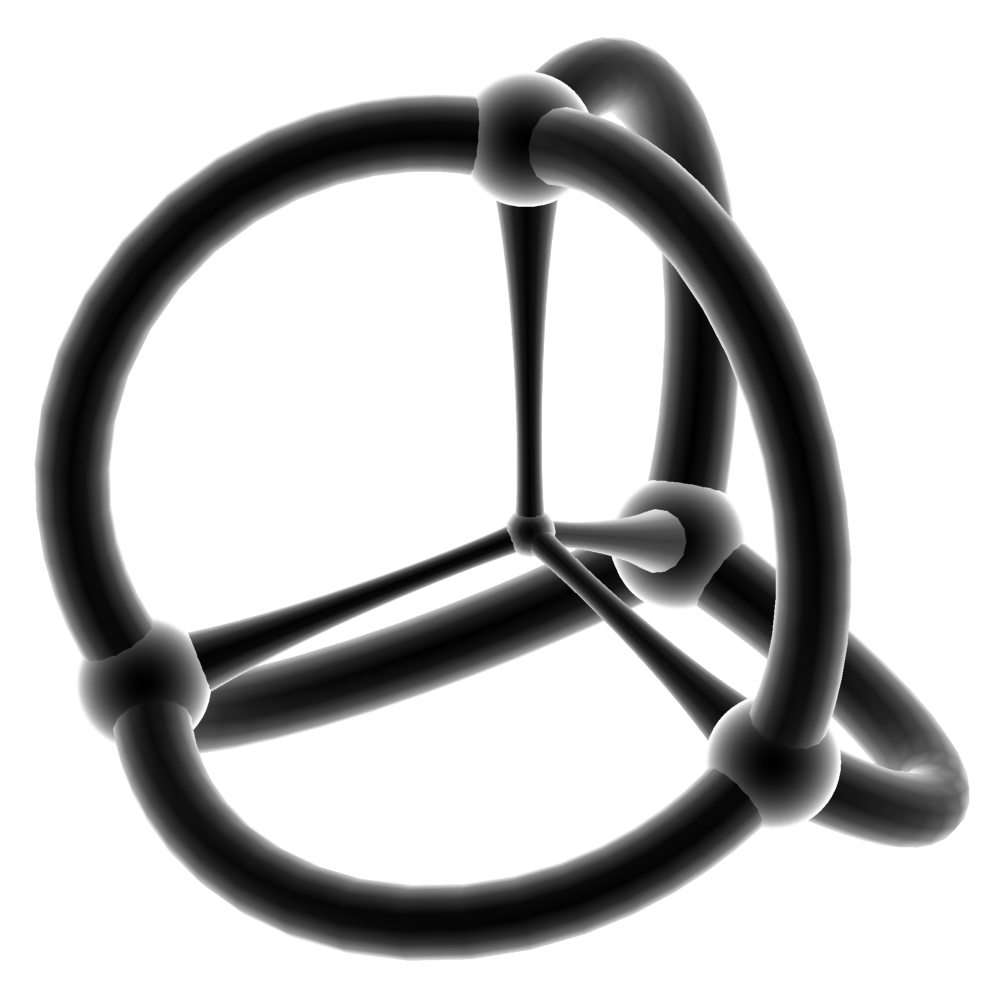
\includegraphics[width=4cm]{matematika/obrazky/4simplex.png}
\caption{Pentachoron}
\end{center}
\end{figure}

Nyn� p�istupme k form�ln� definici �lohy line�rn�ho programov�n�.

\medskip
\ramcek{14cm}{
\noindent{\bf\textsf{�loha line�rn�ho programov�n�}} \\
Je d�n konvexn� polytop v prostoru $\mathbb{R}^n$ popsan� $m$ nerovnostmi.
Maticov� to m��eme zapsat ve tvaru $Ax\leq b$, kde $A$ je re�ln� matice
��du $m\times n$ a $b$ je vektor $m$ re�ln�ch ��sel. D�le je d�n vektor
$c\in\mathbb{R}^n$. Funkce, kterou chceme maximalizovat, je $\sum_{i=1}^n c_ix_i$,
neboli vektorov� $c^Tx$.
Je�t� nav�c hled�me pouze mezi body se v�emi sou�adnicemi
nez�porn�mi (tj. $x_i\geq 0$ pro $i=1,\dots, n$).
}

\noindent\textsf{Terminologie}
\begin{penumerate}
 \item Vektoru $c$ ��k�me {\it cenov� vektor}, funkci $c^Tx$ pak {\it ��elov� funkce}.
 \item Nerovnosti $Ax\leq b$ a $x\geq 0$ jsou {\it omezuj�c� podm�nky}, vektor $b$ je {\it prav� strana �lohy}.
 \item Konkr�tn� zad�n� �lohy line�rn�ho programov�n� (tj. matice $A$ a vektory $b$, $c$) je {\it p��pustn�},
pokud existuje n�jak� bod spl�uj�c� $x\geq 0$ a $Ax\leq b$. Jinak je zad�n� {\it nep��pustn�}.
 \item �loha je {\it neomezen�}, pokud m��eme ��elovou funkc� dos�hnout na p��pustn�ch bodech libovoln� velik� hodnoty.
Jinak je {\it omezen�}.
\end{penumerate}

\begin{e}{V�ta}{0}{0}
Pro p��pustnou a omezenou �lohu line�rn�ho programov�n�\,\footnote{Tedy existuje alespo� jedno �e�en�
a ��elov� funkce je shora omezen�.} existuje bod, ve kter�m ��elov� funkce nab�v� maxima. T�chto
bod� obecn� m��e b�t v�ce a ��k�me jim optim�ln� �e�en�.
\end{e}

\subsection{Simplexov� metoda}

Simplexov� metoda je ozna�en� pro algoritmus �e��c� �lohu line�rn�ho programov�n�. Byla publikov�na
v roce 1947 jedn�m ze zakladatel� line�rn�ho programov�n� ameri�anem Georgem Dantzigem.

\medskip
\begin{center}
{\bf\textsf{Idea}}
\end{center}
\ramcek{14cm}{
Zkonstruujeme p��pustn� �e�en� v n�kter�m vrcholu polytopu. Pot� jdeme po hran�ch do vrchol�
s vy��� hodnotou ��elov� funkce.}

Omezuj�c� podm�nku $Ax\leq b$ tedy zm�n�me na $Ax=b$. Toho doc�l�me p�id�n�m jedn� nez�porn� prom�nn� pro ka�dou podm�nku ( $\sum{x}<b$ je toti� ekvivalentn� $\sum{x}+y=b$ kde $y\in\mathbb{R}^+$). Tuto �pravu lze tak� zapsat jako $A:=(A\ I)$. D�le p�edpokl�d�me, �e matice $A$ m� line�rn� nez�visl� ��dky.
Pro podmno�inu index� $I\subseteq \{1, 2, \dots, n\}$
ozna�me $A_I$ matici $A$, ze kter� ponech�me pouze sloupce, kter� jsou v~$I$. Analogicky pro libovoln� vektor $w\in\mathbb{R}^n$
ozna�me jako $w_I$ vektor, z n�ho� ponech�me jenom sou�adnice z~$I$ (m� dimenzi $n-|I|$).

\ramcek{14cm}{
{\it B�ze} (a to nem� nic spole�n�ho s b�z� vektorov�ho prostoru) je libovoln� podmno�ina index� $B\subseteq \{1, 2, \dots, n\}$ takov�, �e matice $A_B$ je regul�rn�.
Nav�c �ekneme, �e b�ze je {\it p��pustn�}, pokud rovnice $A_Bx_B=b$ m� nez�porn� �e�en�.
Vektor $x\in\mathbb{R}^n$ je tzv. {\it bazick� �e�en�}\,\footnote{N�kdy t� b�zov� �e�en�.}, pokud existuje b�ze $B$ takov�, �e
$A_Bx_B=b$ a $x_i=0$ pro ka�d� $i\in\{1,2,\dots,m\}\backslash B$.
}
Poznamenejme jen, �e bazick� �e�en� je�t� nemus� b�t p��pustn�. Je-li nav�c i p��pustn�,
��k�me mu p�irozen� {\it p��pustn� bazick� �e�en�}. Prom�nn�m $x_j$ pro $j\in B$, kde
$B$ je b�ze, ��k�me bazick�.

\begin{e}{V�ta}{0}{0}
Nech� $x\in\mathbb{R}^n$ je p��pustn� �e�en�. Pak $x$ je bazick� �e�en�, pr�v� kdy�
sloupce matice $A$ odpov�daj�c� kladn�m prom�nn�m jsou line�rn� nez�visl�.
\end{e}
%\begin{e}{D�kaz}{0}{0}
%Jako $K$ ozna�me mno�inu t�ch index�, pro kter� je $x_j>0$. Implikace $\Rightarrow$ je jednoduch�,
%nebo� je-li $x$ bazick� �e�en�, pak existuje b�ze $B$ tak, �e $A_B$ je regul�rn� a $x_{[n]\backslash B}=0$.
%Jeliko� jsou ale v�echny sou�adnice $x$ vn� $B$ nulov�, je nutn� $K\subseteq B$, a tedy $A_K$ je rovn� regul�rn�.
%Nyn� uka�me implikaci $\Leftarrow$.
%\end{e}

\begin{e}{V�ta}{0}{0}
Nech� $B$ je $m$--prvkov� indexov� mno�ina $B\subseteq \{1,\dots, n\}$ a $A_B$ je regul�rn�. Pak existuje
nejv��e jedno p��pustn� bazick� �e�en� $x$ ($x_i\neq 0 \Leftrightarrow i\in B$).
\end{e}

Mezi prvn� tvrzen�mi jsme uvedli, �e m�-li dan� �loha line�rn�ho programov�n� n�jak� p��pustn�
�e�en� a je-li z�rove� ��elov� funkce na mno�in� p��pustn�ch �e�en� omezen�, pak existuje
optim�ln� �e�en� (tj. nab�v� se maxima). D� se ale dok�zat dokonce n�sleduj�c�.

\ramcek{14cm}{
\begin{e}{V�ta}{0}{0}
M�-li dan� �loha optim�ln� �e�en�, pak i n�kter� bazick� �e�en� je optim�ln�.
\end{e}}
Tato v�ta m� obrovskou d�le�itost, nebo� je jasn�, �e {\bf bazick�ch �e�en� je jen kone�n� mnoho}.
Uka�me si fungov�n� simplexov� metody na konkr�tn�m p��kladu.
\begin{e}{P��klad}{0}{0}
Maximalizujte funkci $z(x_1,\dots,x_5) = x_1+x_2$ za omezuj�c�ch podm�nek $x_i\geq 0$ ($i=1,\dots, 5$) a
\begin{center}
\fbox{
\begin{tabular}{rrrrrl}
$-x_1$ & $+x_2$ & $+x_3$ & & & $=1$     \\
$+x_1$ & & & $+x_4$ &  & $=3$       \\
& $+x_2$ & & & $+x_5$ & $=2$       \\
\end{tabular}}
\end{center}
\end{e}

\begin{proof}[�e�en�]
Nejprve najdeme libovoln� p��pustn� bazick� �e�en�. Matice $A$ a vektor $b$ t�to �lohy jsou ze zad�n�
\[
A=
\left(
\begin{array}[h]{ccccc}
-1 & 1 & 1 & 0 & 0      \\
1 & 0 & 0 & 1 & 0       \\
0 & 1 & 0 & 0 & 1
\end{array}\right),\quad
b=\left(\begin{array}[h]{c}
   1 \\ 3 \\ 2
  \end{array}\right)
\]
a $m=3, n=5$. Vid�me tedy, �e jedn�m z bazick�ch �e�en� je $R_1 = (0,0,1,3,2)^T$. Odpov�daj�c�
b�ze index� je $B=\{3,4,5\}$ (matice $A_B$ je jednotkov�, a tedy regul�rn�). Na z�klad� tohoto
vytvo��me tzv. {\it simplexovou tabulku} (po��te�n� p��pustnou tabulku) tak, �e vyj�d��me bazick� prom�nn�
pomoc� nebazick�ch a p�id�me jeden ��dek s vyj�d�enou ��elovou funkc� pomoc� nebazick�ch prom�nn�ch.
\[
\begin{array}{c|ccc}
x_3=& 1 & +x_1 & -x_2   \\
x_4=& 3 & -x_1 &        \\
x_5=& 2 & & -x_2        \\
\hline
z=& & x_1 & +x_2
\end{array}, \quad R_1 = (0,0,1,3,2)^T, \quad z=0
\]

V bod� $R_1$ je $z(R_1) = 0$. Nyn� budeme, jak bylo nazna�eno, postupn� zvy�ovat
hodnotu funkce $z$, dokud nezjist�me, �e jsme nalezli optim�ln� �e�en�. Hodnotu funkce $z$ budeme
zv�t�ovat zv�t�en�m hodnoty n�kter� nebazick� (voln�) prom�nn�.

Ponechejme $x_1=0$ a zv�t�eme $x_2$ z $0$ na $1$ (jedni�ka je nejlep�� mo�n�, viz prvn� rovnici a $x_3\geq 0$).
Pak pomoc� tabulky dostaneme nov� p��pustn� �e�en�, konkr�tn� $R_2=(0,1,0,3,1)^T$. Z prvn� rovnice te�
vyj�d��me $x_2$:
\[
x_2 = 1+x_1-x_3
\]
a nahrad�me touto rovnic� p�vodn� prvn� rovnici $x_3=1+x_1-x_2$. Toto �e�en� odpov�d� b�zi $B=\{2,4,5\}$.
Snadno zjist�me, �e $z(R_2) = 0+1 = 1$. Nyn� se stalo, �e prom�nn� $x_2$ nahradila prom�nnou $x_3$ v b�zi.
Tomuto procesu ��k�me, �e prom�nn� $x_2$ \uv{vstoupila do b�ze}, $x_3$ z n� \uv{vystoupila}.
\smallskip

Dost�v�me tak novou simplexovou tabulku
\[
\begin{array}{c|ccc}
x_2=& 1 & +x_1 & -x_3   \\
x_4=& 3 & -x_1 &        \\
x_5=& 1 & -x_1& +x_3        \\
\hline
z=& 1& +2x_1 & -x_3
\end{array}, \quad R_2=(0,1,0,3,1)^T, \quad z=1
\]
Nyn� budeme zvy�ovat $x_1$. Prvn� rovnice $x_1$ neomezuje, druh� ��k� $x_1\leq 3$ a t�et� nyn� ��k� $x_1\leq 1$
(jeliko� $x_3=0$). Polo�me tedy $x_1=1$. Dost�v�me nov� �e�en� $R_3=(1,2,0,2,0)^T, z(R_3) = 3$. Prom�nn�
$x_1$ vstoup� do b�ze m�sto prom�nn� $x_5$. Nov� b�ze je $B=\{1,2,4\}$.
\smallskip

Dost�v�me dal�� simplexovou tabulku
\[
\begin{array}{c|ccc}
x_1=& 1 & +x_3 & -x_5   \\
x_2=& 2 &  &  -x_5       \\
x_4=& 2 & -x_3& +x_5        \\
\hline
z=& 3& +x_3 & -2x_5
\end{array}, \quad R_3=(1,2,0,2,0)^T, \quad z=3
\]
Zv�t��me $x_3$ z $0$ na $2$ ($x_3\leq 2$ plyne ze t�et� rovnice tabulky) a t�m obdr��me
dal�� �e�en� $R_4=(3,2,2,0,0)^T$, b�ze je $B=\{1,2,3\}$, $z(R_4)=5$. Odpov�daj�c� nov�
simplexov� tabulka je
\[
\begin{array}{c|ccc}
x_1=& 3 & -x_4 &    \\
x_2=& 2 &  &  -x_5       \\
x_3=& 2 & -x_4& +x_5        \\
\hline
z=& 5& -x_4 & -x_5
\end{array}, \quad R_4=(3,2,2,0,0)^T, \quad z=5
\]
Nyn� je jasn�, �e libovoln� zv��en� voln� prom�nn� $x_4$ nebo $x_5$ sn�� hodnotu ��elov� funkce.
Z konstrukce simplexov� metody plyne, �e �e�en� $R_4$ je ji� optim�ln�, nebo� jsme prov�d�li pouze
ekvivalentn� rovnicov� �pravy. Optim�ln�m �e�en�m dan� �lohy je tedy bod $(3,2,2,0,0)$.



\end{proof}




�asov� slo�itost simplexov� metody je $O(2^n)$.
Jeden z nejhor��ch p��pad� m��eme vz�t $n$--dimenzion�ln� krychli,
kter� m� p�esn� $2^n$ vrchol�. Na t�to krychli algoritmus
m��e postupn� nav�t�vit v�echny jej� vrcholy. 

Simplexov� metoda nach�z� uplatn�n� p�ev�n� p�i �e�en� optimaliza�n�ch �loh v in�en�rstv� nebo ekonomii.

\subsection{Du�ln� �loha}

Probl�m line�rn�ho programov�n� tak, jak byl pops�n v��e, ozna�ujeme jako {\it prim�rn�}.
Ke ka�d�mu prim�rn�mu probl�mu m��eme zkonstruovat {\it du�ln� �lohu}. P�ipome�me, �e
prim�rn� �loha byla naj�t
\[
\max\{ c^Tx : x\in\mathbb{R}^n, Ax\leq b, x\geq 0 \}.
\]
Du�ln� �loha k t�to pak je naj�t
\[
\min\{ b^Ty : y\in\mathbb{R}^m, A^Ty\geq c, y\geq 0 \}.
\]
Z�kladem teorie duality line�rn�ho programu jsou n�sleduj�c� dv� v�ty -- {\it (Slab�) v�ta o dualit�}.

\begin{e}{V�ta}{0}{Slab� v�ta o dualit�}
Pokud je $x$ p��pustn� �e�en� prim�rn� �lohy a $y$ p��pustn� �e�en� du�ln� �lohy, pak
hodnota du�ln� ��elov� funkce v bod� $y$ je alespo� tak velik� jako hodnota prim�rn� ��elov�
funkce v bod� $x$.
\end{e}

\begin{e}{V�ta}{0}{V�ta o dualit�}
Nech� $x_*$ je optim�ln� �e�en� prim�rn� �lohy. Pak existuje optim�ln� �e�en� $y_*$ du�ln� �lohy takov�, �e
\[
c^Tx_* = b^Ty_*.
\]
\end{e}
\bigskip

\noindent{\bf\textsf{Du�ln� �loha ze �ivota}}

\dots 

%M�jme malou pek�rni�ku na rohu ulice a �kola�ku Ka�enku, kter� si chce koupit
%n�co dobr�ho ke~sva�in�. V pek�rni�ce prod�vaj� dva druhy zbo�� -- b�bovky a pa��sk� dorty.
%B�bovka stoj� 80 K�, pa��sk� dort 50 K�. Pek�rn��ku vlastn� jedna hodn� pan� ze sousedstv�, a proto
%si m��ete vz�t i jen kousek b�bovky nebo dort�ku. Na pa��sk� dort�k jsou pot�eba
%3 unce �okol�dy, 2 unce cukru a 2 unce kr�mu. Na b�bovku pak jsou pot�eba
%4 unce cukru a 5 unc� kr�mu. Jeliko� ale Ka�enka d� na spr�vnou v��ivu,\footnote{A da�� se j� to p�evelice.}
%v�, �e mus� j�st hodnotn�, a proto si stanovila, �e chce, aby jej� sva�inka m�la alespo� 6
%unc� �okol�dy, 10 unc� cukru a 8 unc� kr�mu. Jeliko� m� ale malinkatou pen�enku, do kter� se j�
%neve�elo moc pen�zk�, chce, aby si sva�inku spl�uj�c� dan� krit�ria nakoupila co nejlevn�ji.
%Pom��ete mil� Ka�ence?
%\medskip


%Zave�me nyn� $m$ nov�ch prom�nn�ch $x_{n+1}, x_{n+2}, \dots, x_{n+m}$ pomoc� vztahu
%\[
%x_{n+i} = b_i - \sum_{j=1}^n A_{ij}x_j,\quad i=1, 2, \dots, m
%\]
%a p�idejme pro ka�dou takto nov� vytvo�enou prom�nnou je�t� omezuj�c� podm�nku $x_{n+i}\geq 0$.
%Ka�d� prom�nn� $x_{n+i}$ je tedy jakousi \uv{chybou} (rozd�lem) hodnoty prav� strany
%a hodnoty lev� strany $i$--t� nerovnosti.


\end{document}
